 
 
\documentclass[a4paper,10pt]{article}
\usepackage[utf8]{inputenc}
\usepackage{listings}
\usepackage[usenames,dvipsnames]{color}
\usepackage{graphicx}
%opening
\title{OT-Med R Mapping Template}
\author{Sinan Shi}
\date{\today}


\lstset{ %
  backgroundcolor=\color{white},   % choose the background color; you must add \usepackage{color} or \usepackage{xcolor}
  basicstyle=\footnotesize\ttfamily,        % the size of the fonts that are used for the code
  breakatwhitespace=false,         % sets if automatic breaks should only happen at whitespace
  breaklines=true,                 % sets automatic line breaking
  captionpos=b,                    % sets the caption-position to bottom
  commentstyle=\color{Violet},     % comment style
  deletekeywords={...},            % if you want to delete keywords from the given language
  escapeinside={\%*}{*)},          % if you want to add LaTeX within your code
  extendedchars=true,              % lets you use non-ASCII characters; for 8-bits encodings only, does not work with UTF-8
%   frame=false,                    % adds a frame around the code
  keepspaces=true,                 % keeps spaces in text, useful for keeping indentation of code (possibly needs columns=flexible)
  keywordstyle=\bfseries\color{blue},       % keyword style
  language=R,                 % the language of the code
  morekeywords={*,...},            % if you want to add more keywords to the set
%   numbers=left,                    % where to put the line-numbers; possible values are (none, left, right)
%   numbersep=5pt,                   % how far the line-numbers are from the code
%   numberstyle=\tiny\color{mygray}, % the style that is used for the line-numbers
  rulecolor=\color{black},         % if not set, the frame-color may be changed on line-breaks within not-black text (e.g. comments (green here))
  showspaces=false,                % show spaces everywhere adding particular underscores; it overrides 'showstringspaces'
  showstringspaces=false,          % underline spaces within strings only
  showtabs=false,                  % show tabs within strings adding particular underscores
  stepnumber=2,                    % the step between two line-numbers. If it's 1, each line will be numbered
  stringstyle=\color{Orange},      % string literal style
  tabsize=2,                       % sets default tabsize to 2 spaces
  title=\lstname                   % show the filename of files included with \lstinputlisting; also try caption instead of title
}


%  \lstset{style=codeStyleR}


\begin{document}

\maketitle
\listoffigures






\begin{figure}
  \centering
    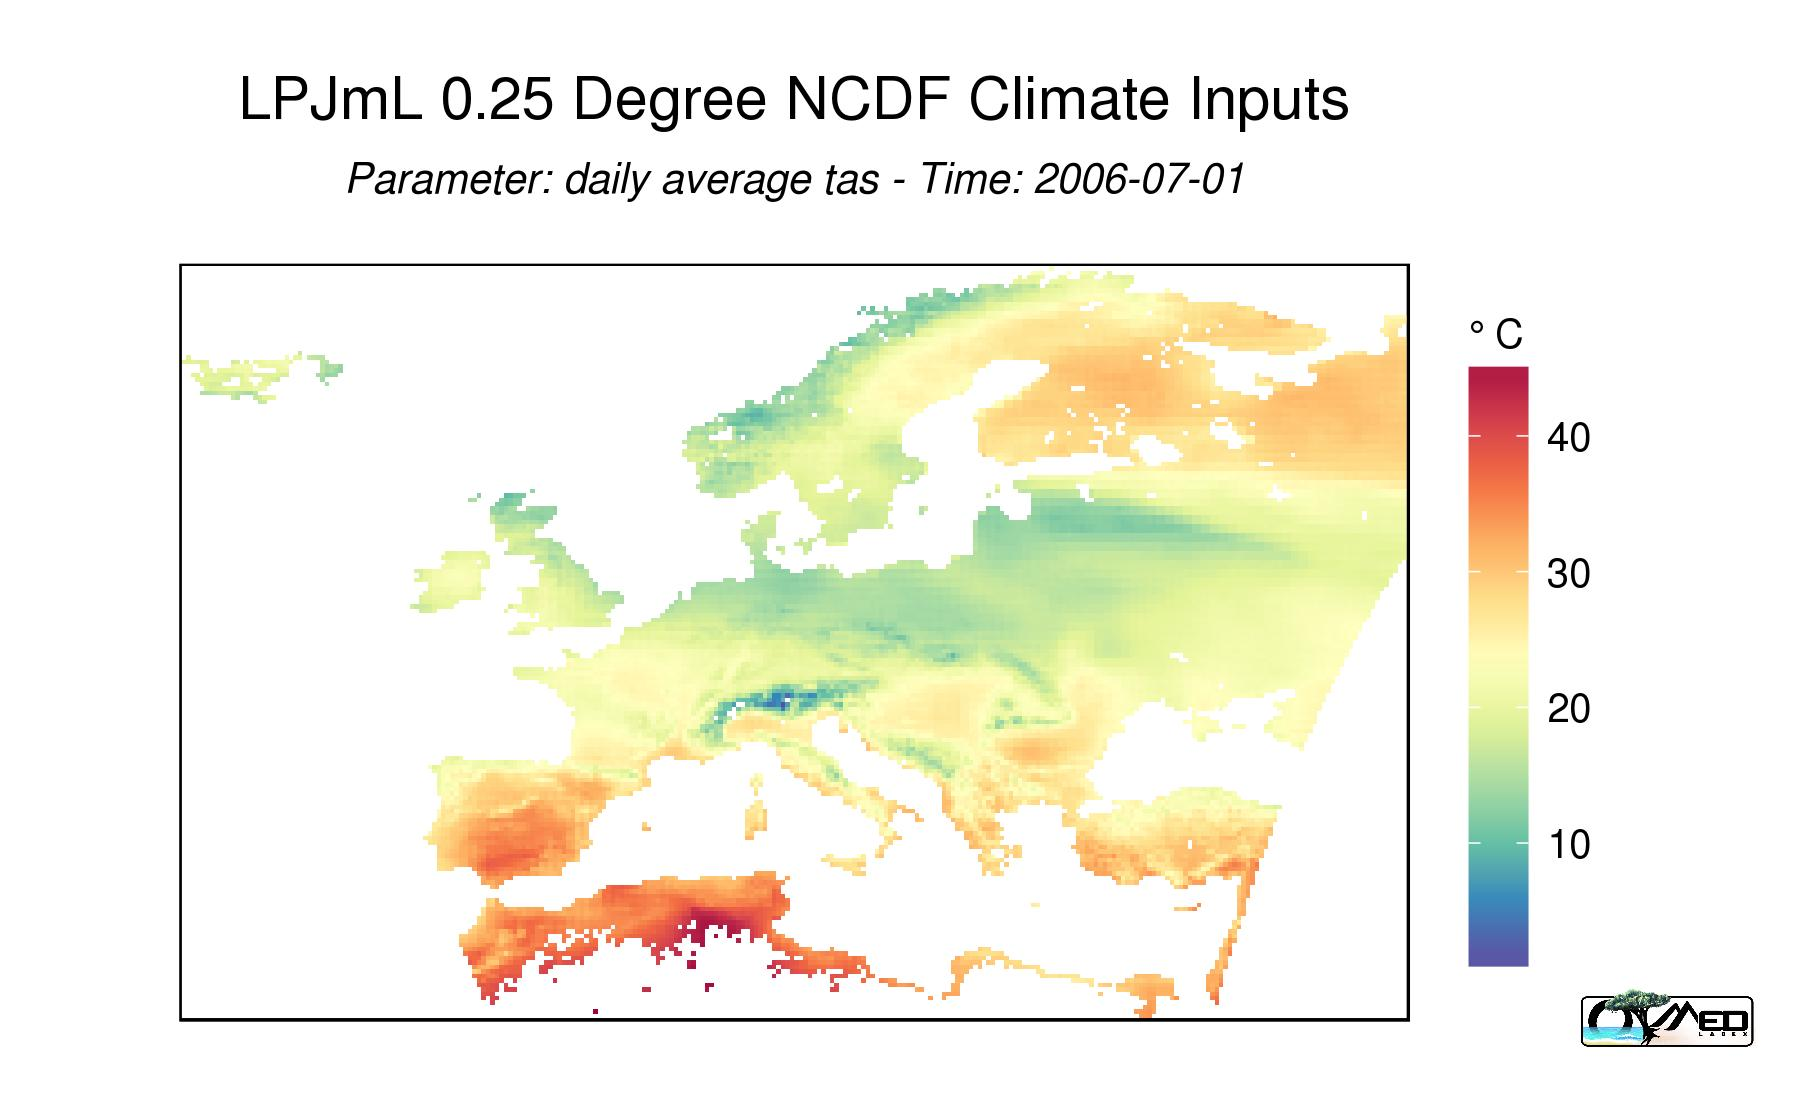
\includegraphics[width=1.2\textwidth]{origin}
  \caption{Original raster data from NCDF}
\end{figure}

\begin{figure}
  \centering
    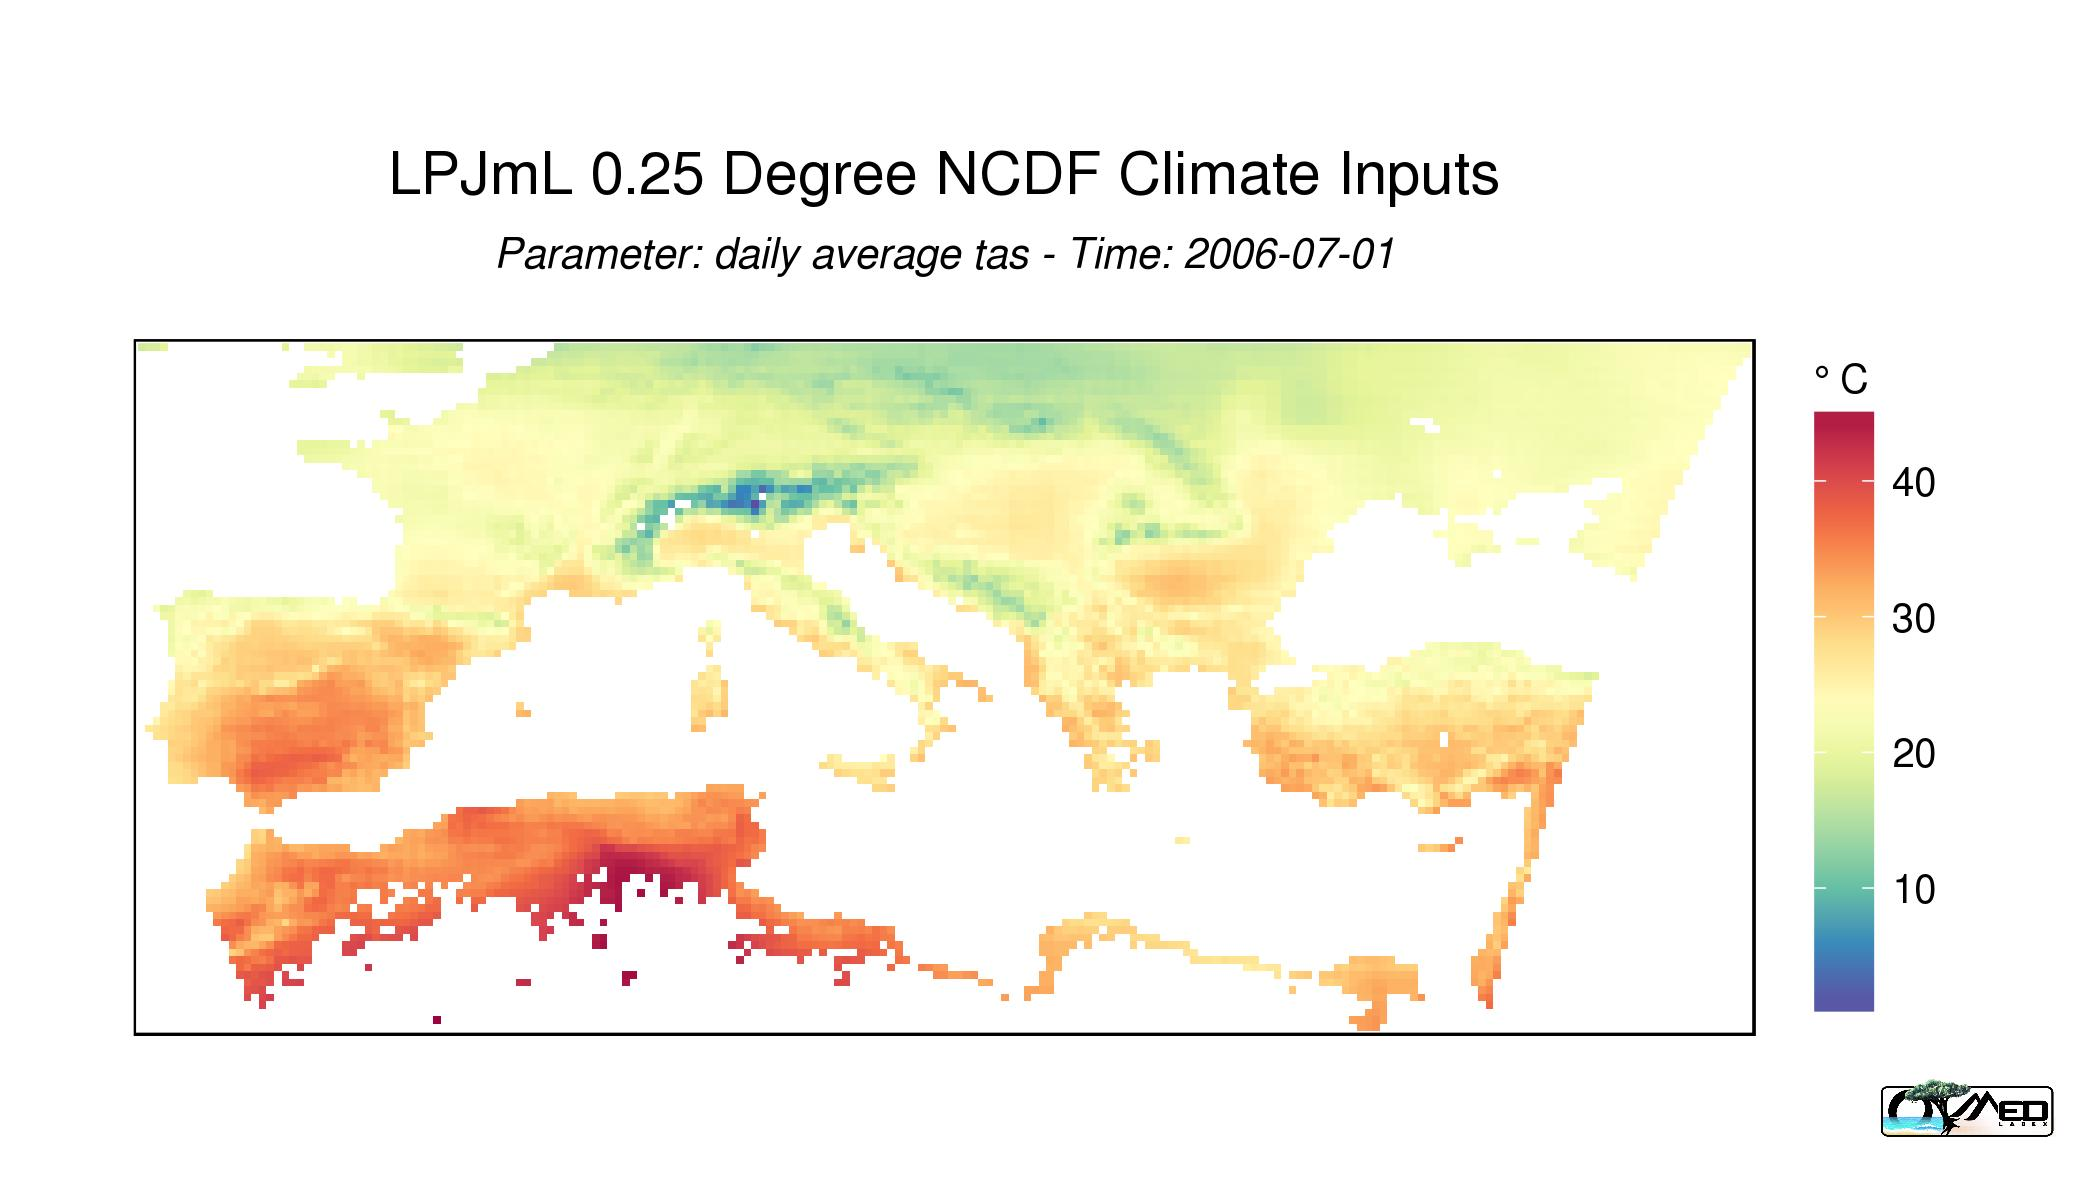
\includegraphics[width=1.2\textwidth]{origin_window}
  \caption{cut\_window: put original data by a user specified boundary}
\end{figure}
\begin{figure}
  \centering
    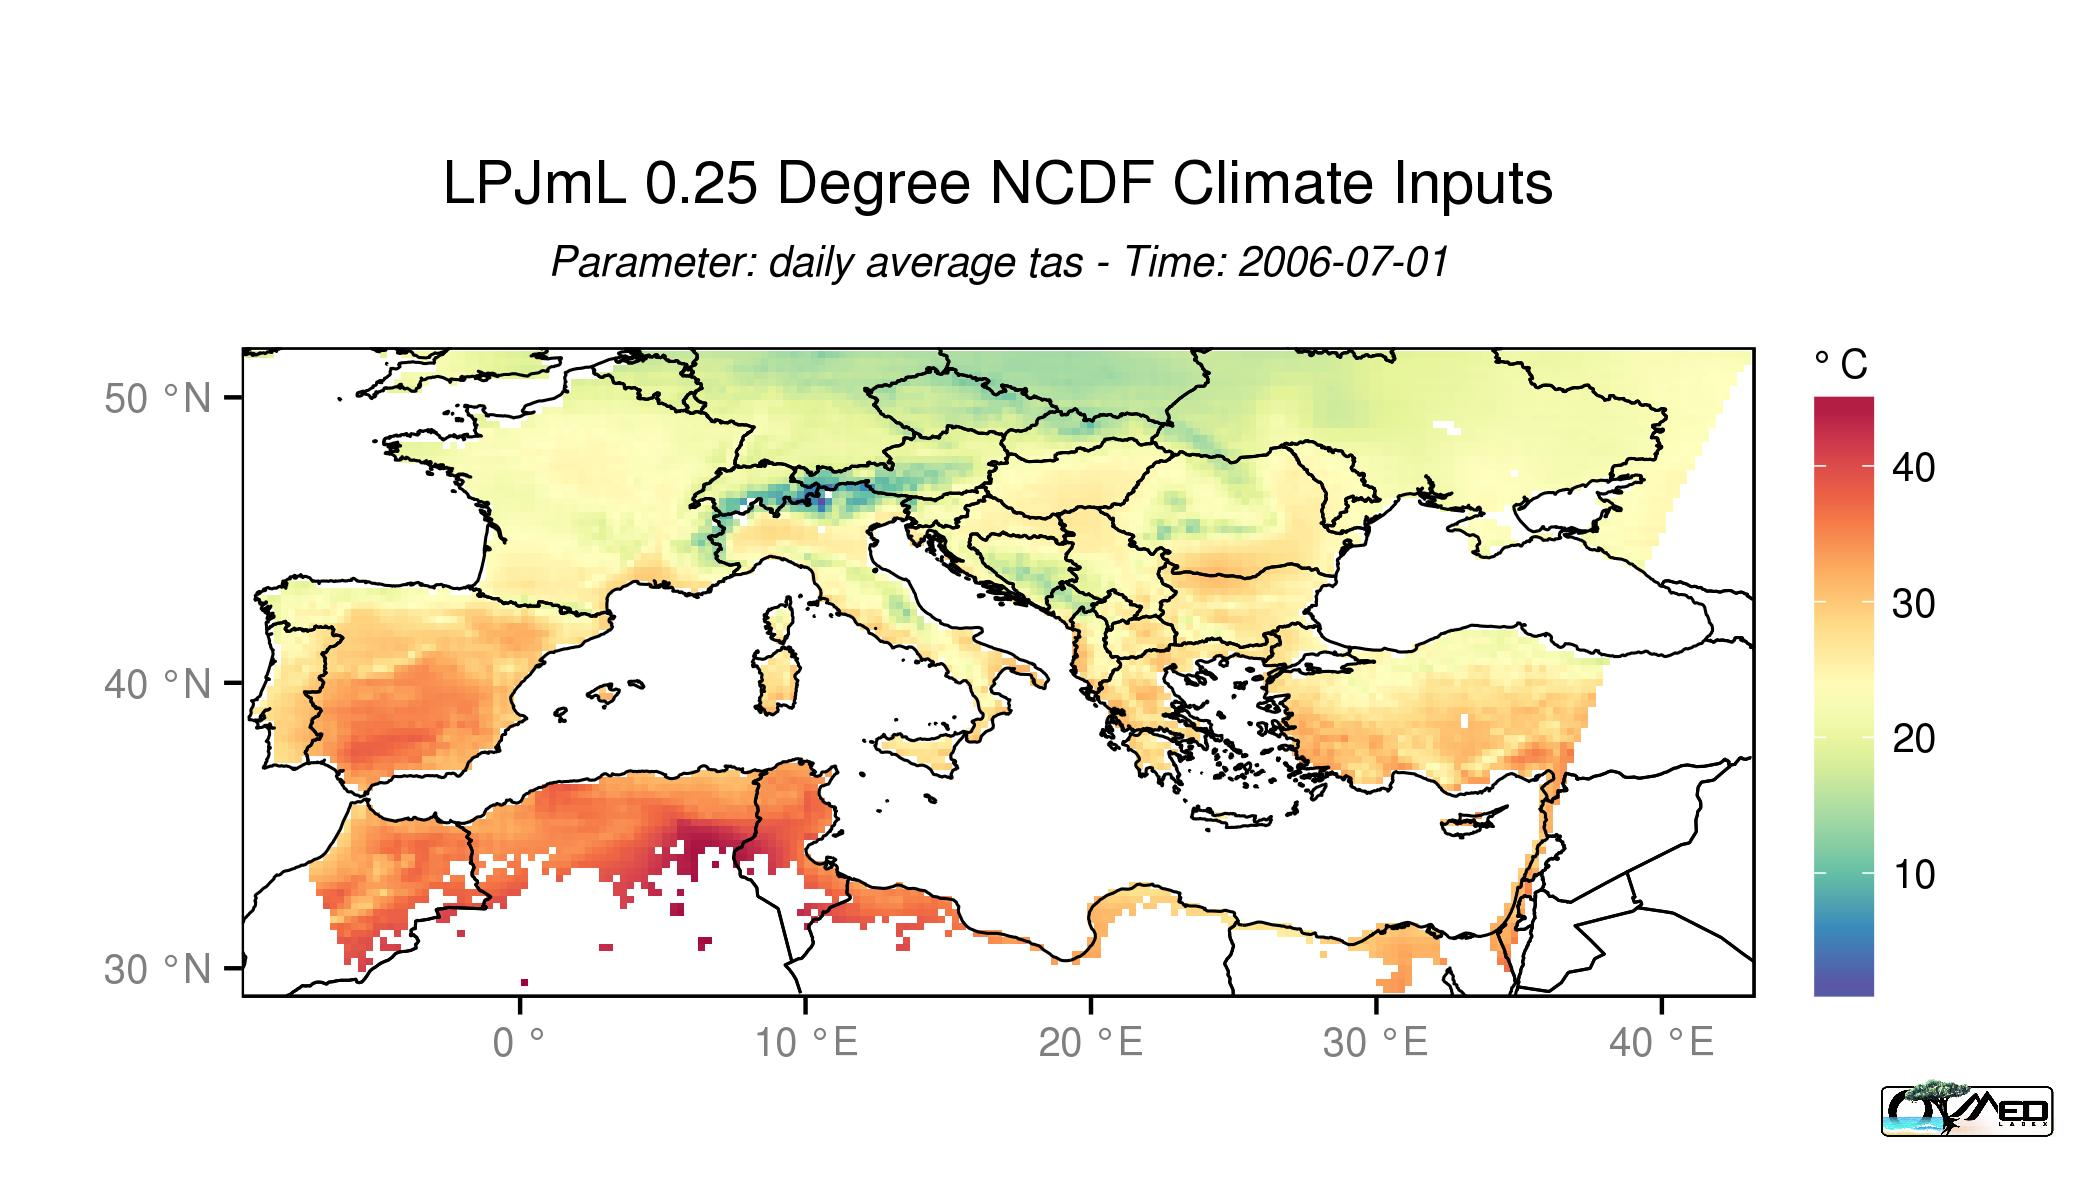
\includegraphics[width=1.2\textwidth]{origin_add_text}
  \caption{addLines: the template has prepared 5 different types of polygon data, including country lines,
	  coastlines, rivers, lakes and islands, all in 3 resolution 10 min, 50 min, 110 min. User defined
	  ESRI Shape files can also be implemented in this function.}
\end{figure}
\begin{figure}
  \centering
    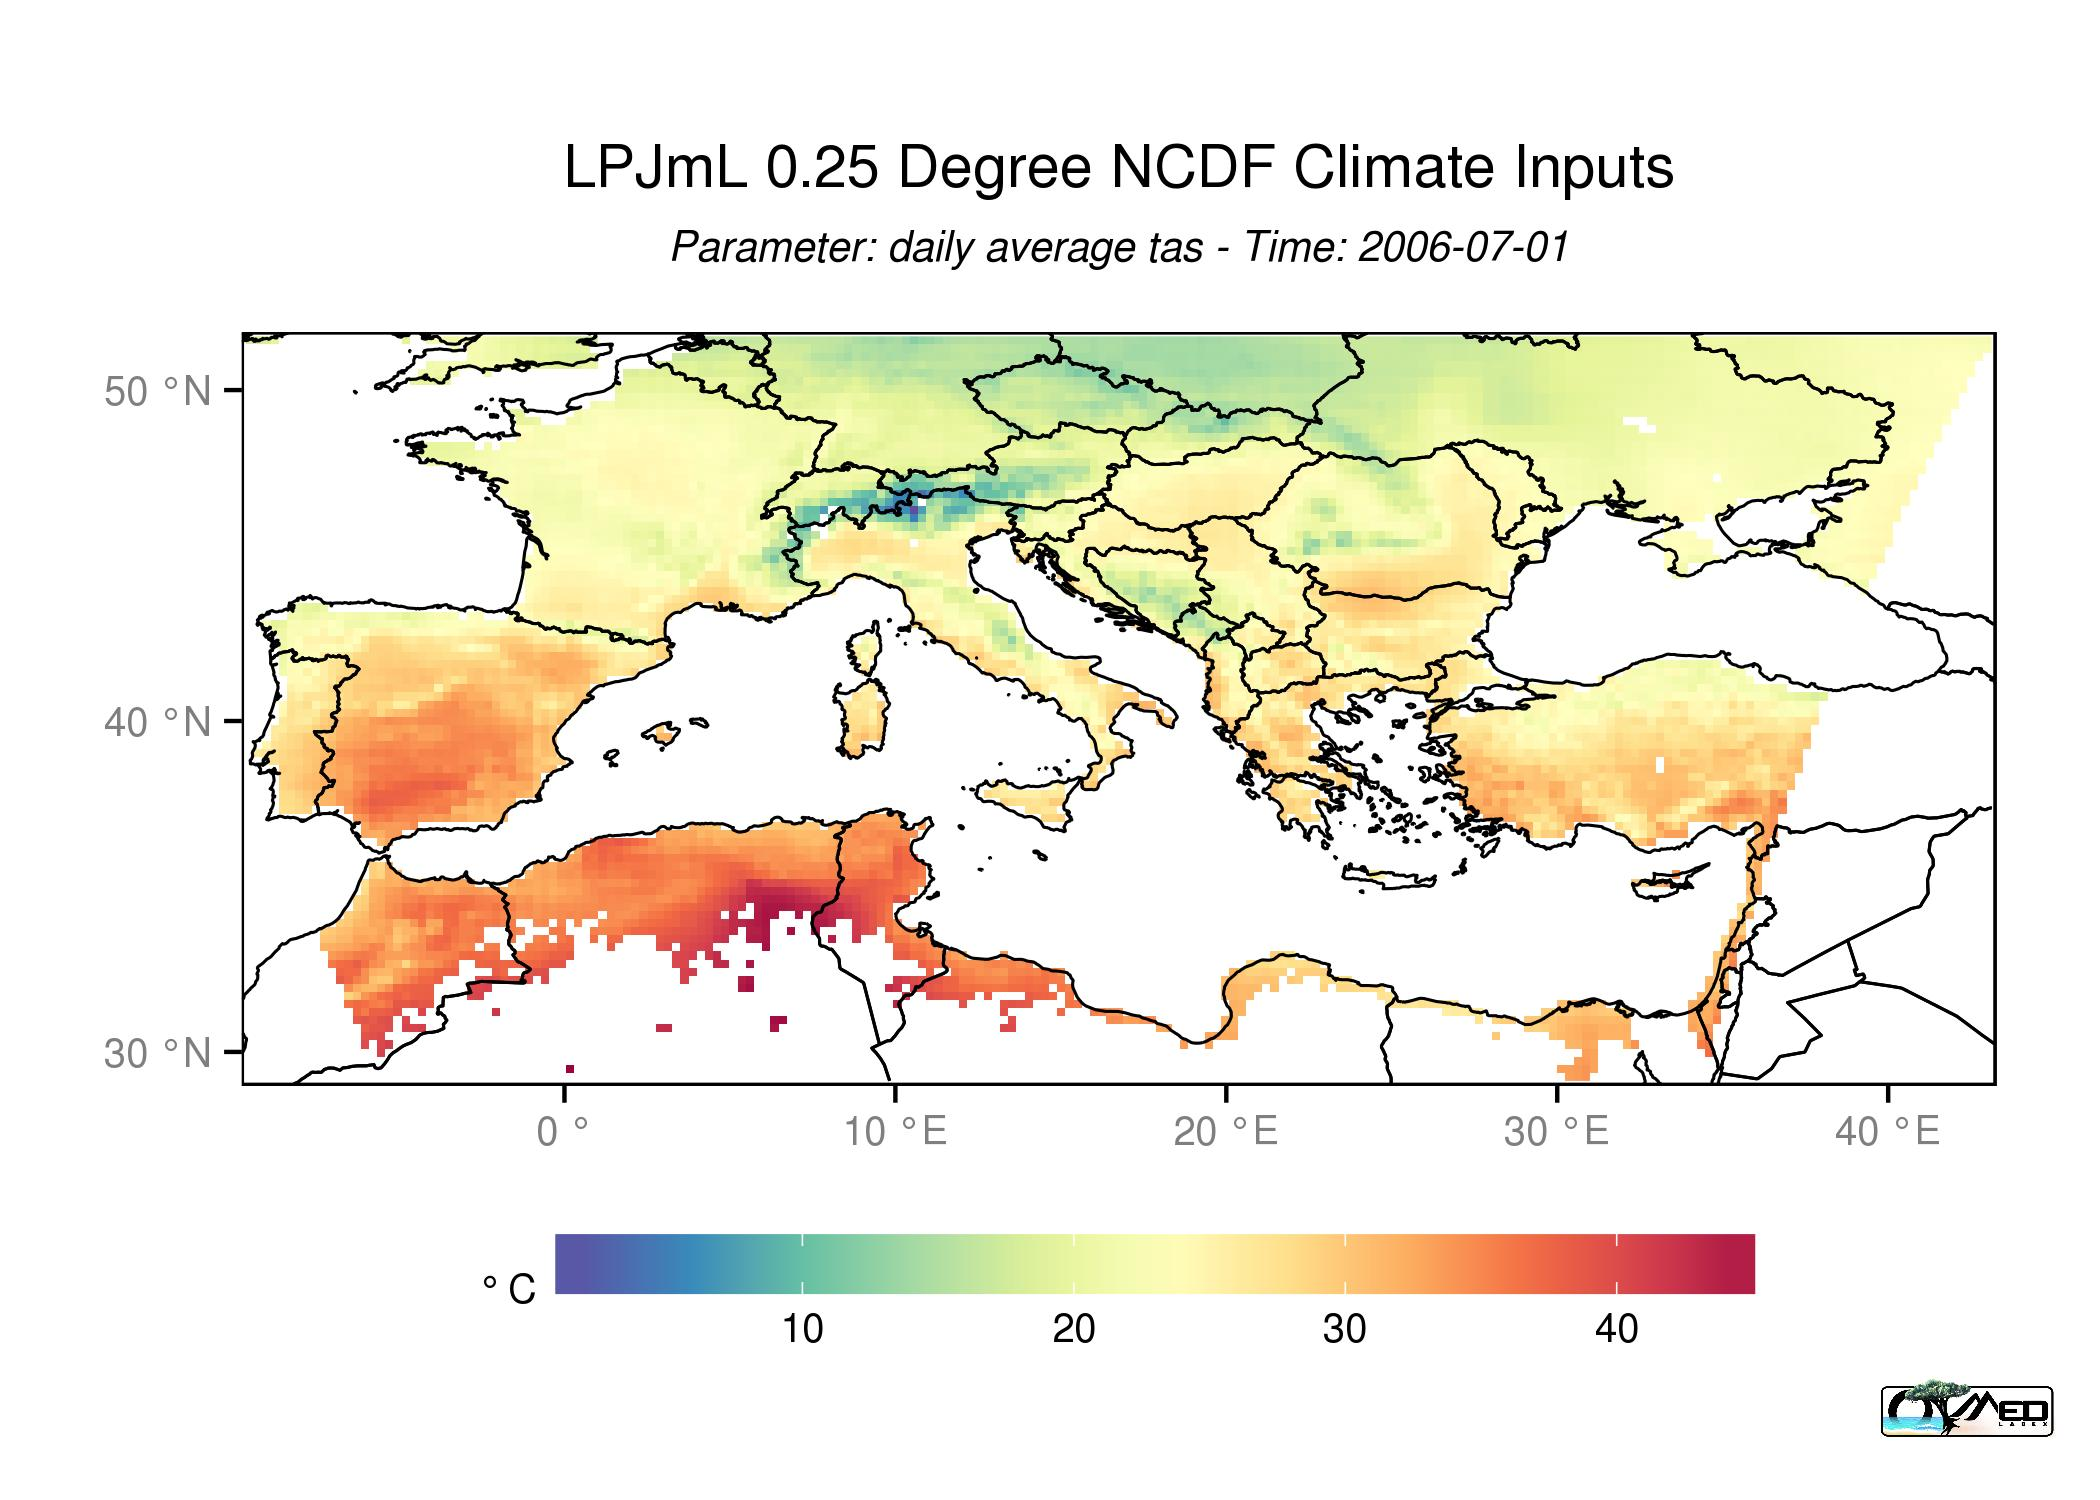
\includegraphics[width=1.2\textwidth]{origin_move_legend}
  \caption{Moving legend position: position can be top, bottom, left and right}
\end{figure}

\begin{figure}
  \centering
    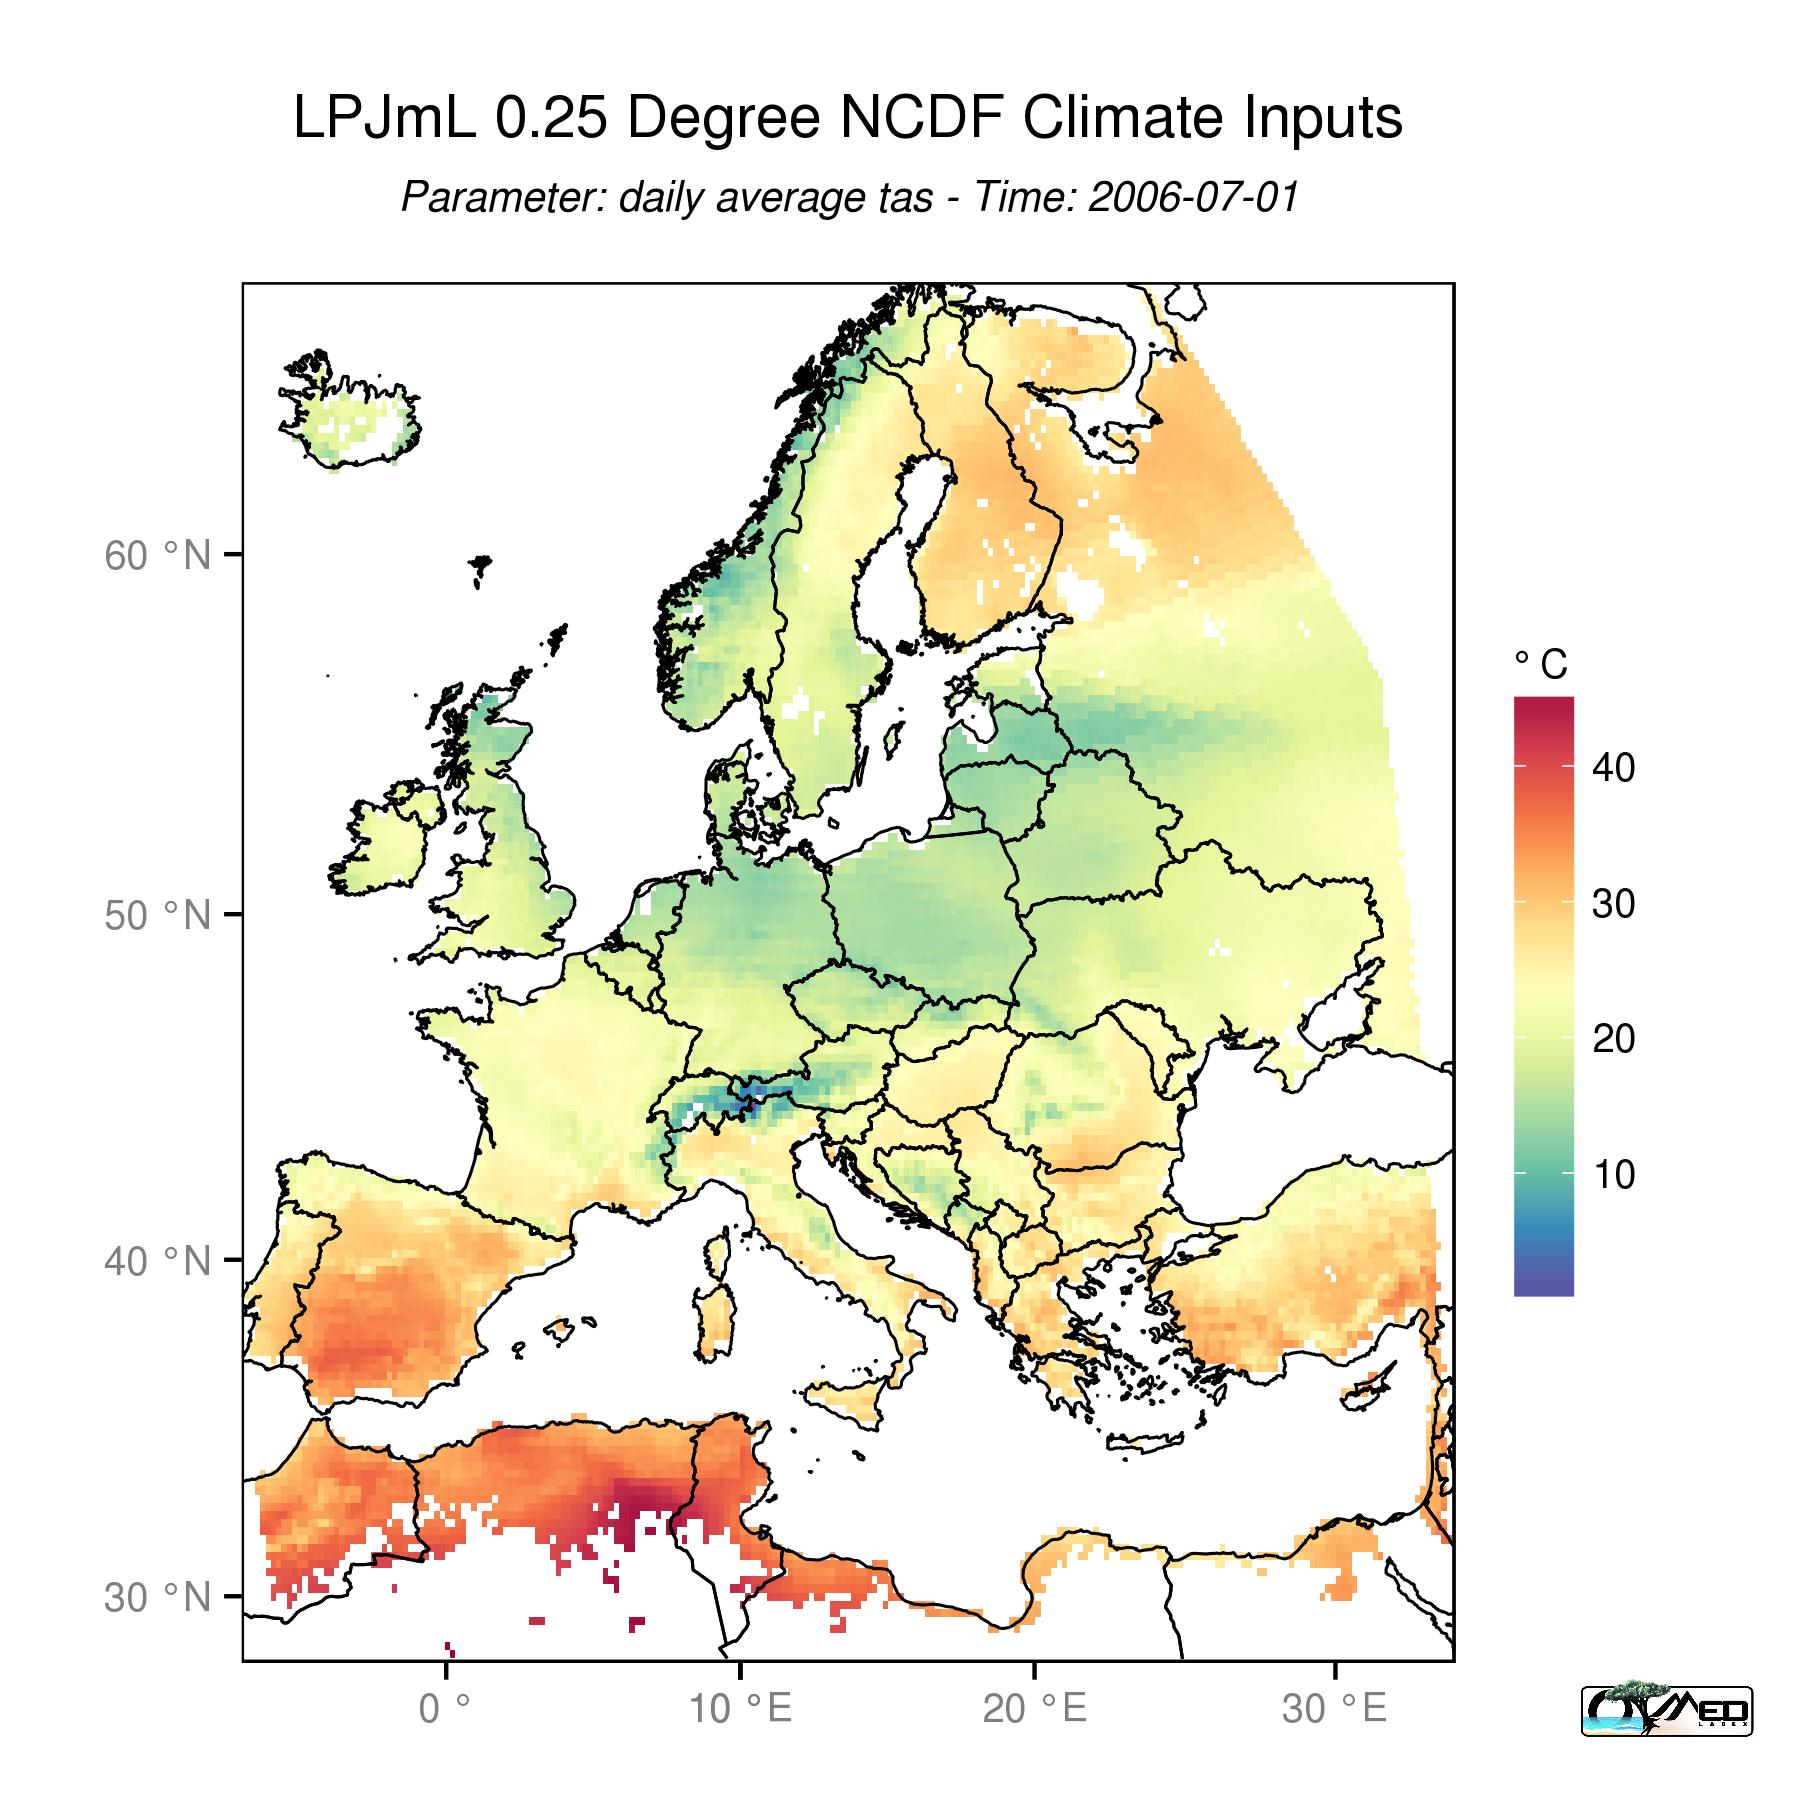
\includegraphics[width=1.2\textwidth]{projections}
  \caption{mapProjection: this function allows user to convert rasters, shape files and points into a 
	  specified projection by proj4 strings.}  
\end{figure}
\begin{figure}
  \centering
    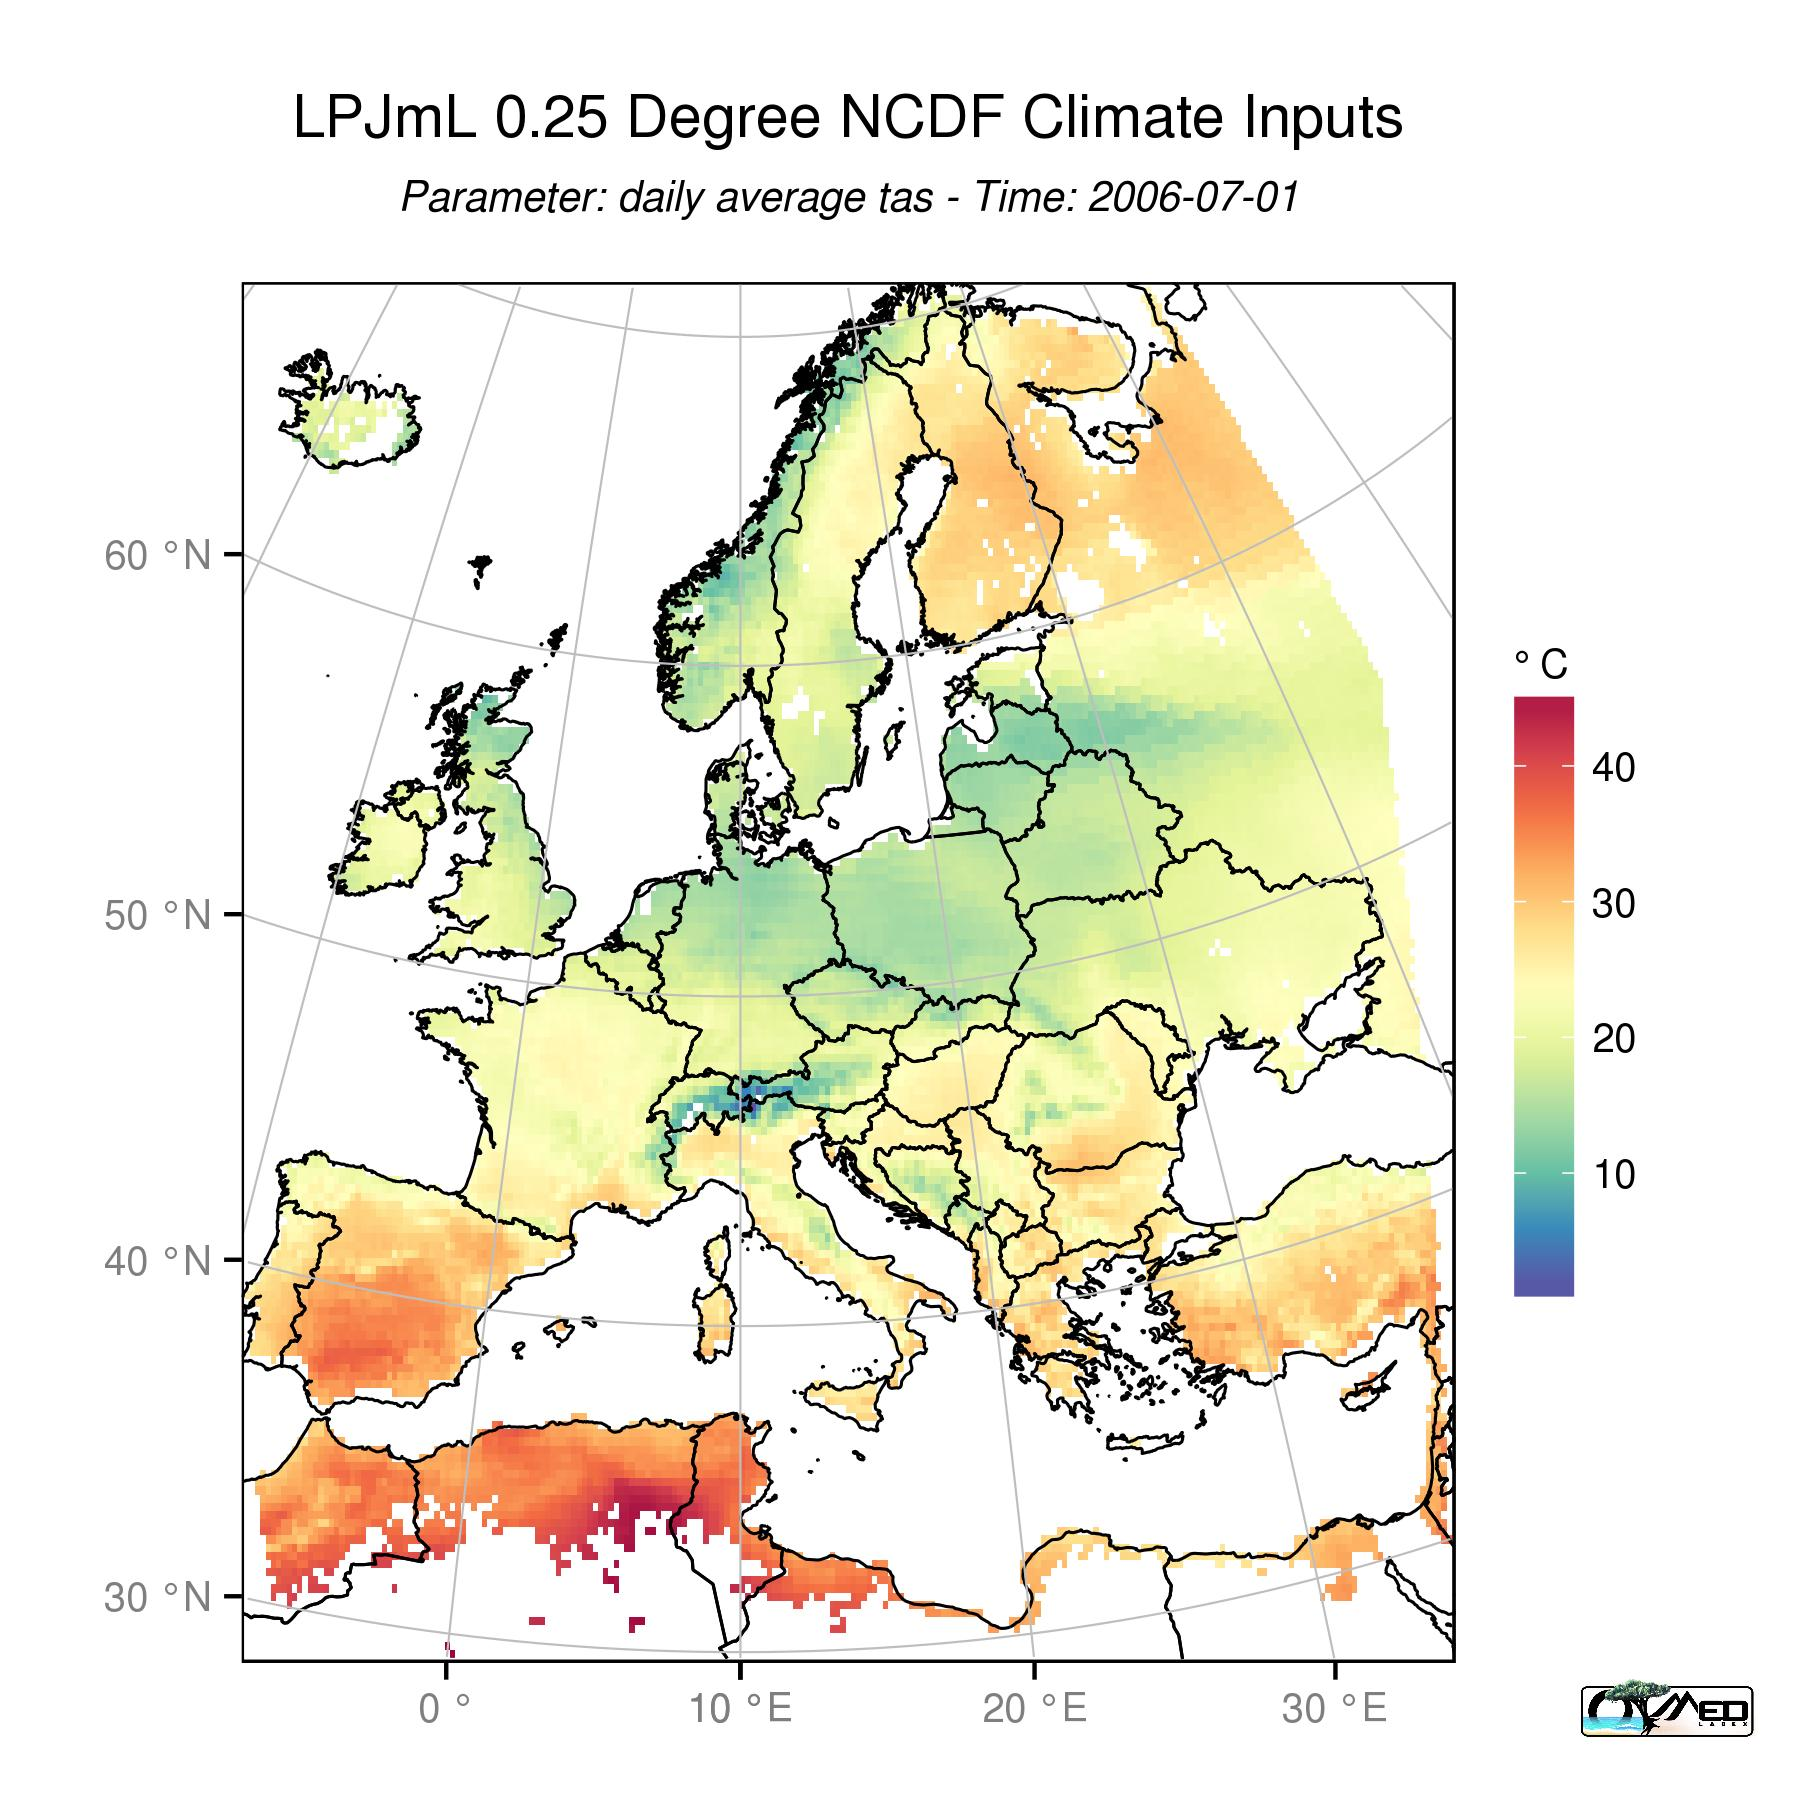
\includegraphics[width=1.2\textwidth]{projection_with_graticules.jpeg}
  \caption{mapProjection: this function allows user to convert rasters, shape files and points into a 
	  specified projection by proj4 strings.}  
\end{figure}

% \begin{figure}
%   \centering
%     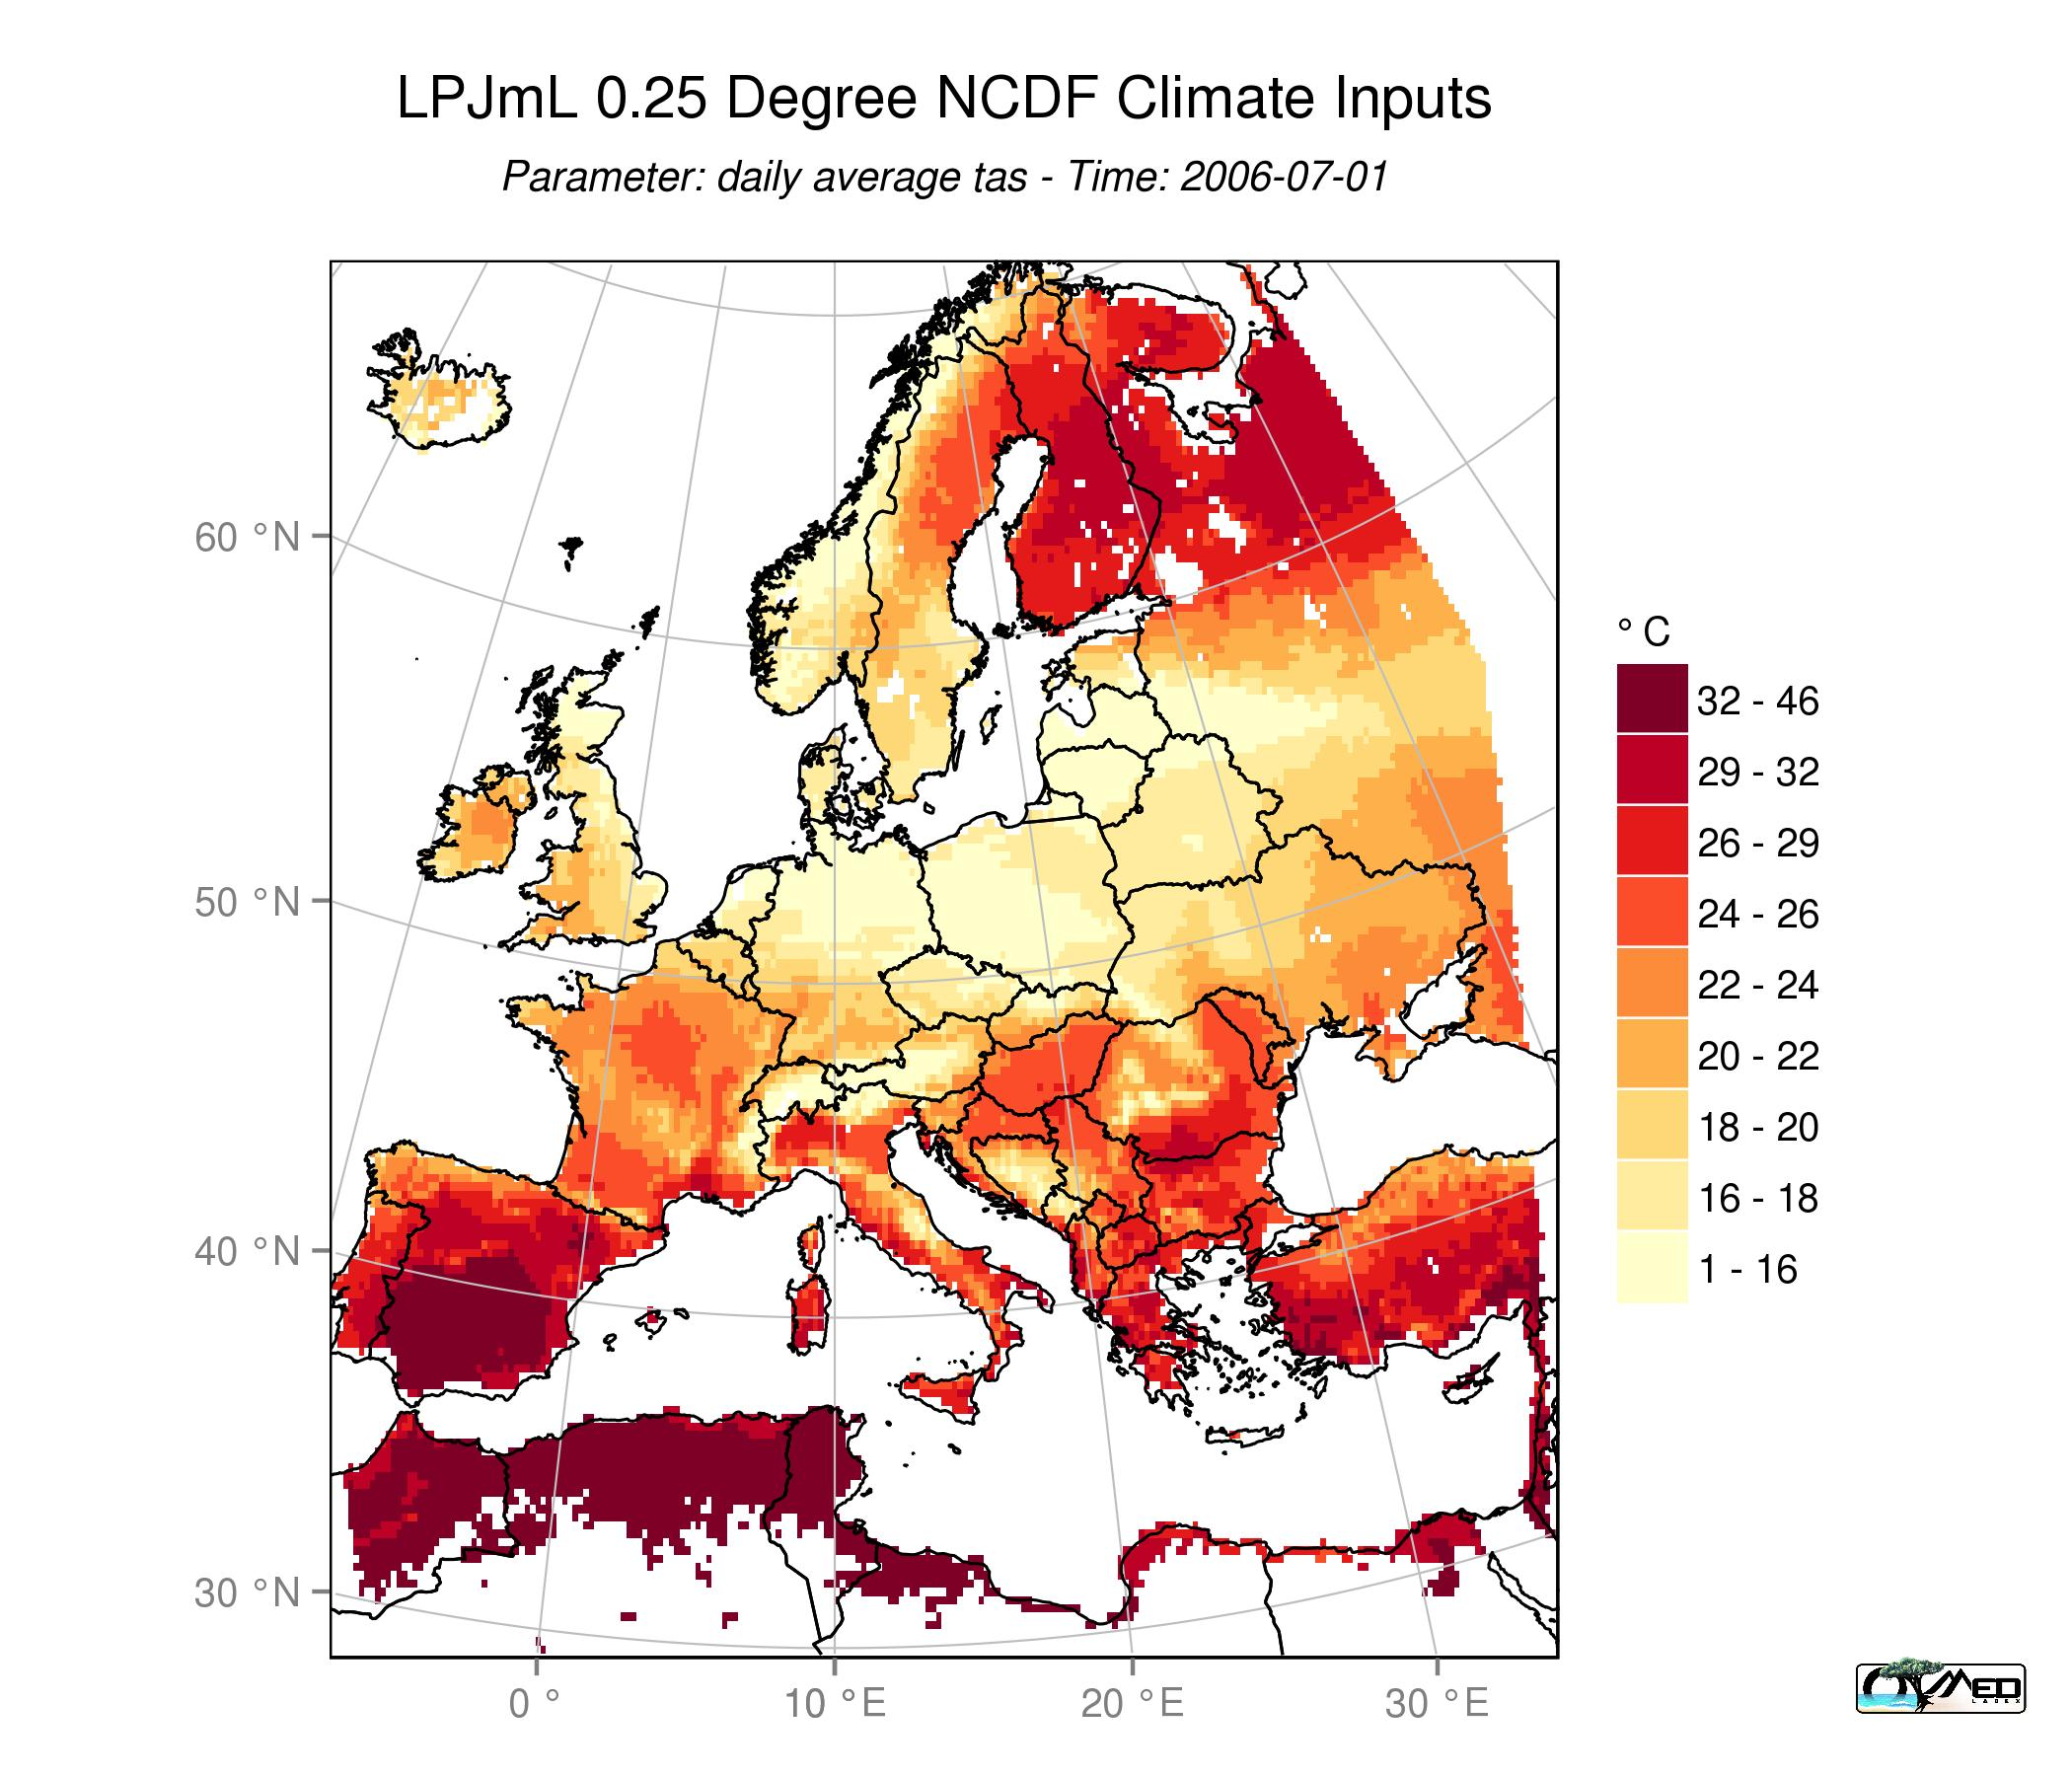
\includegraphics[width=1\textwidth]{std_discrete}
%     \caption{Discrete Colour Scale by Classification of Values}
%   \label{fig:discrete}
% \end{figure}
% 
% 
% 
% \begin{figure}
%   \centering
%     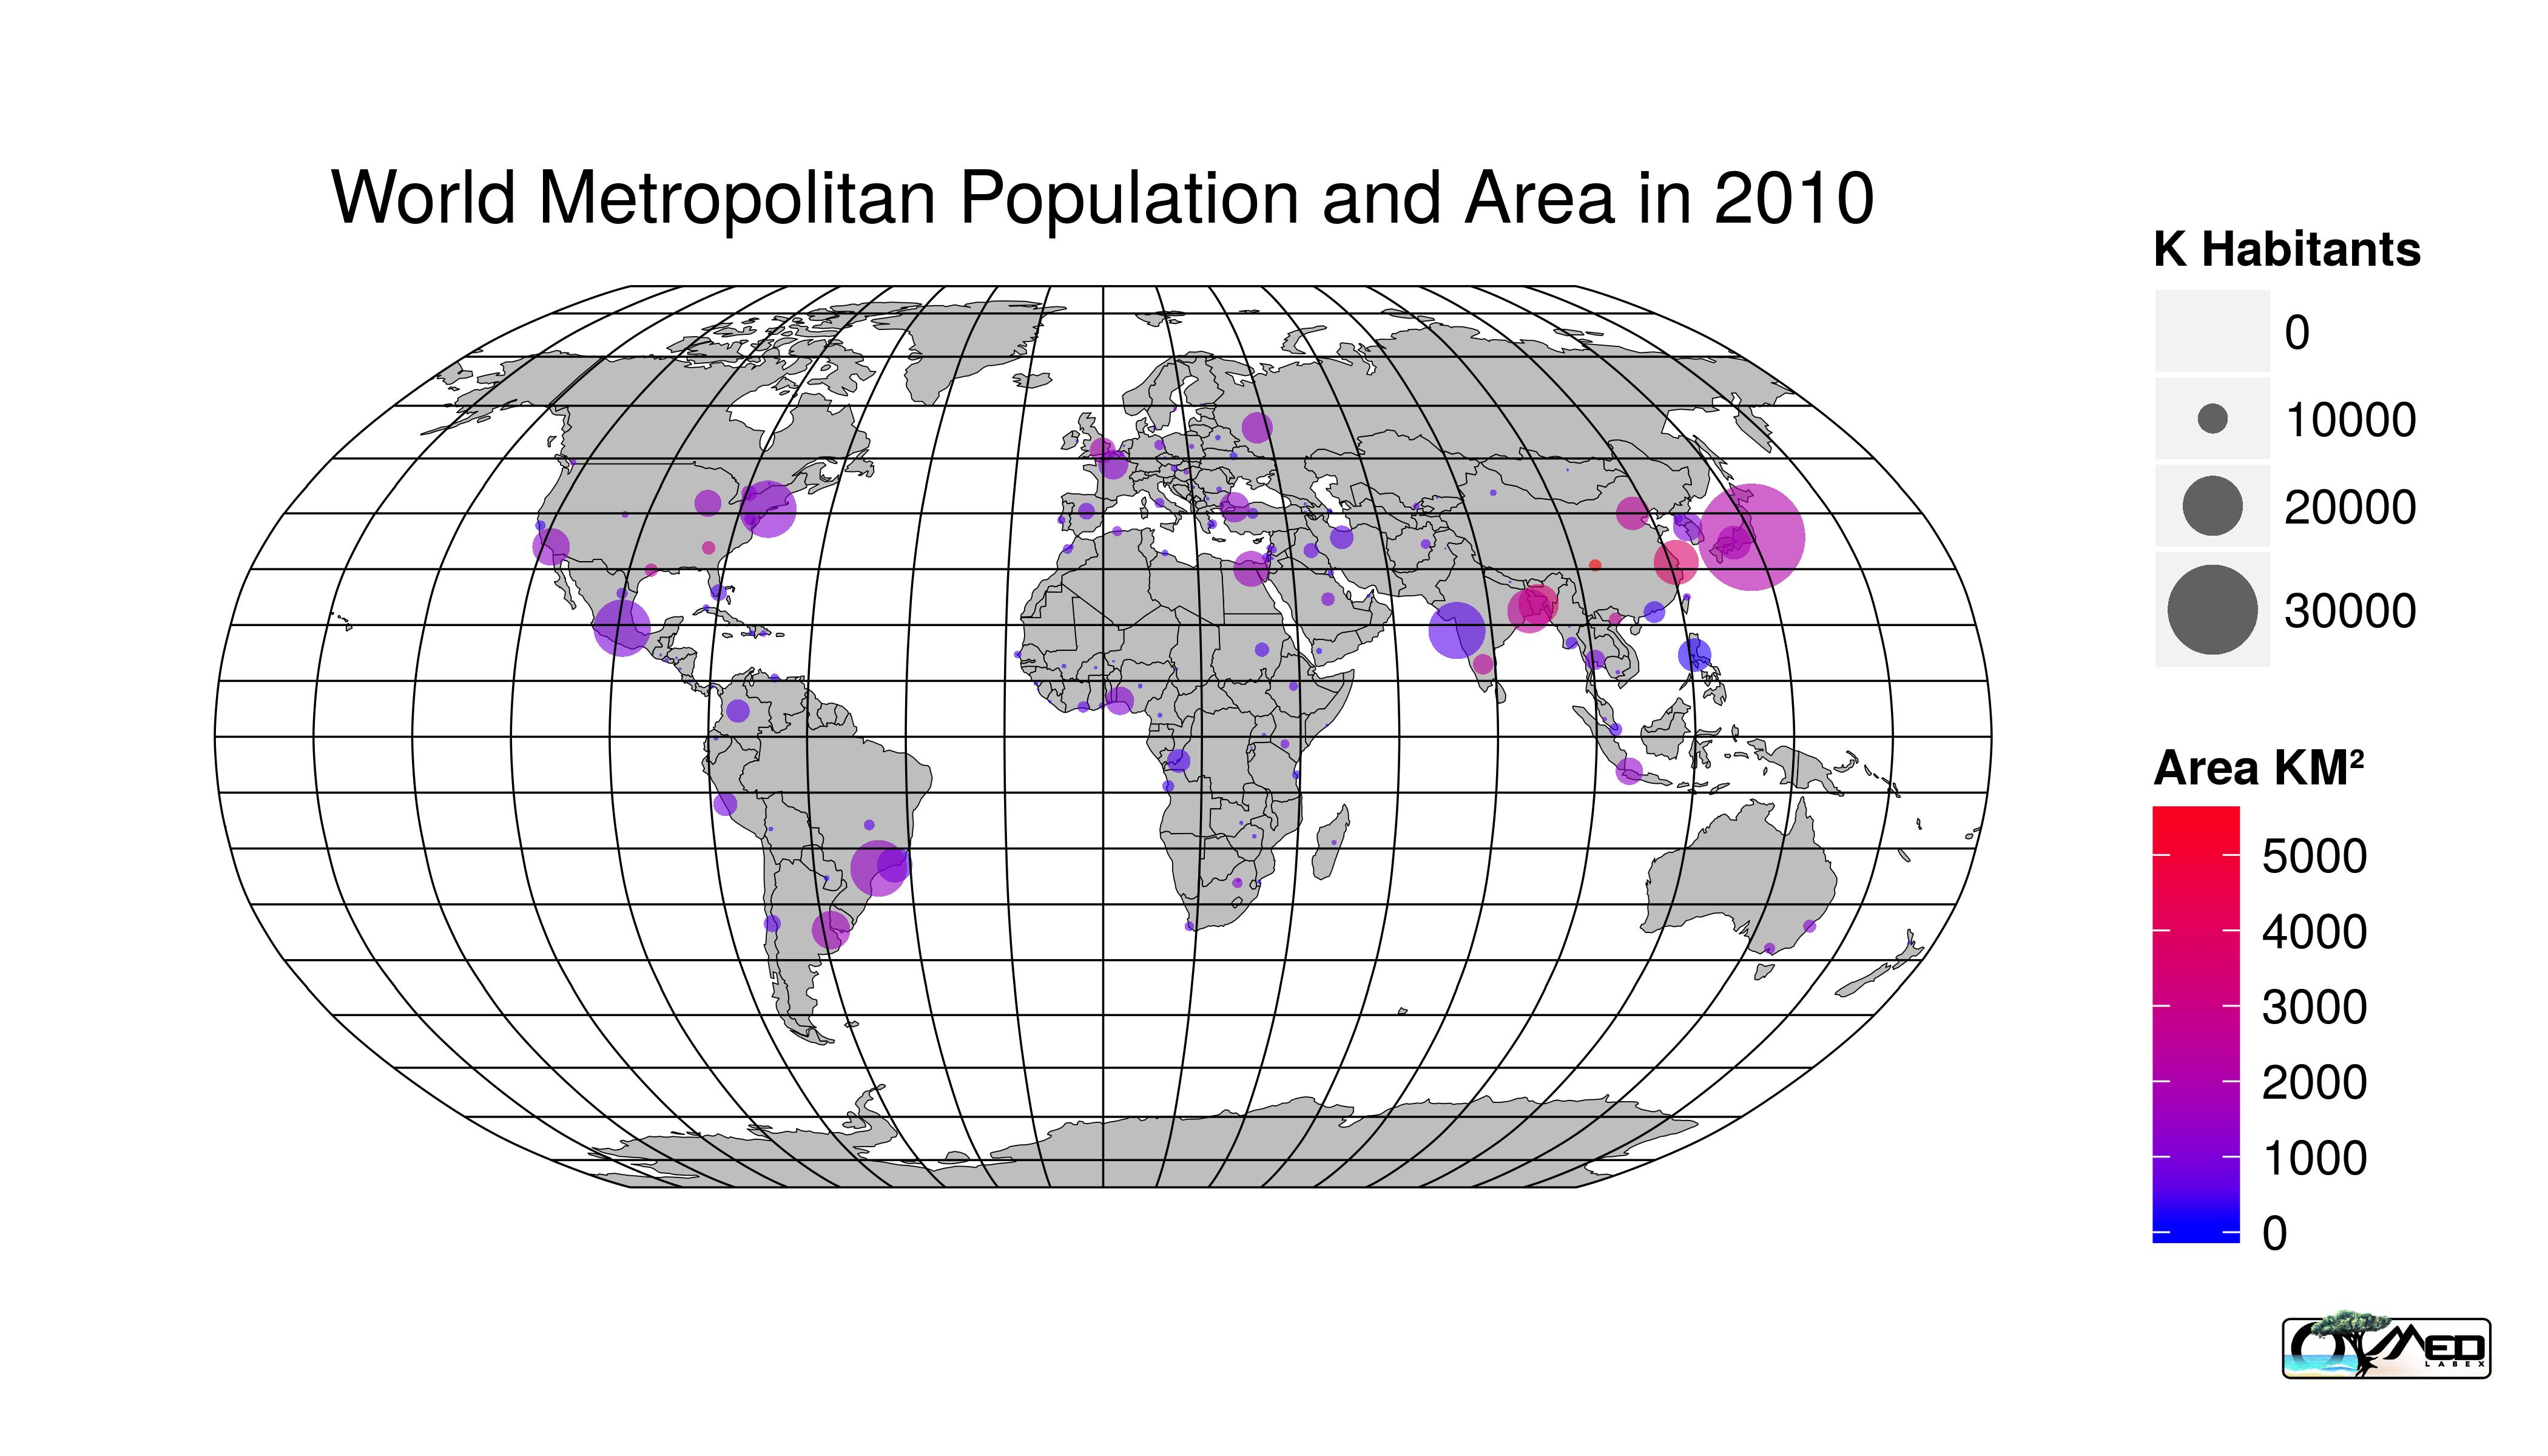
\includegraphics[width=1\textwidth]{point_pj}
%   \caption{Maps from Attributes of Polygons or Spatial Points}
%   \label{fig:point_prj}
% \end{figure}
% 
% 
% 
% 
% 
% \subsection{Standard Map}
% \subsection{Built in Polygons}
% \subsection{Projections}
% \subsection{Selecting Colour Scales}
% 
% \begin{figure}
%   \centering
%    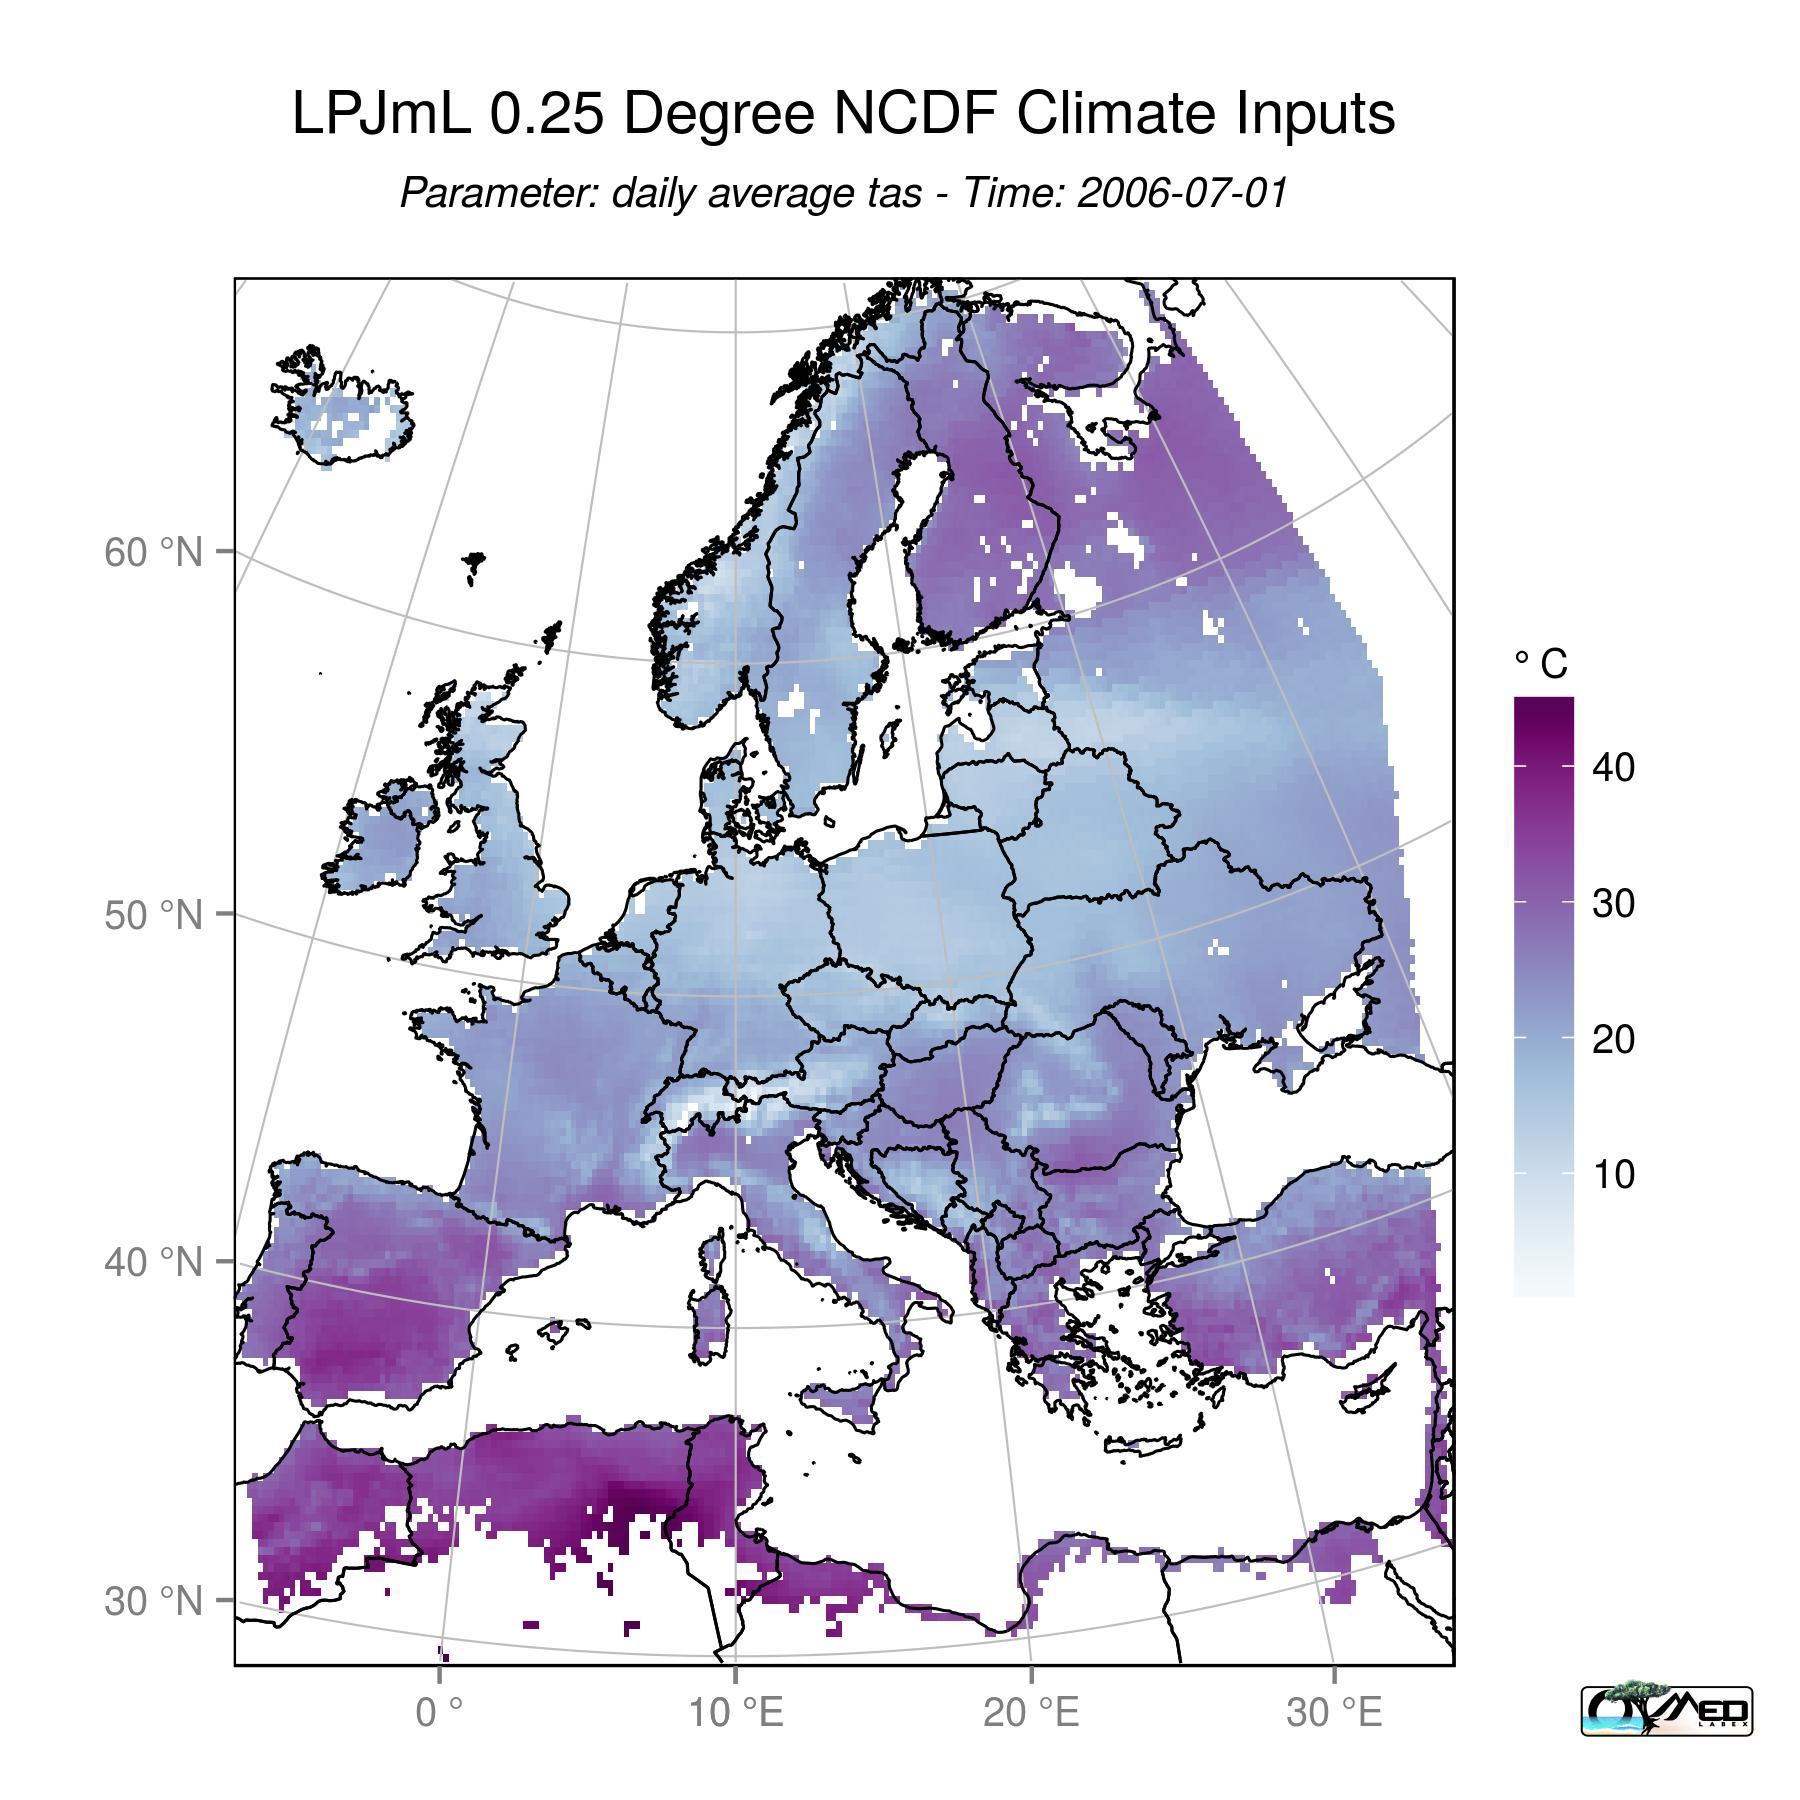
\includegraphics[width=0.45\textwidth, height=0.45\textwidth]{col1}
%   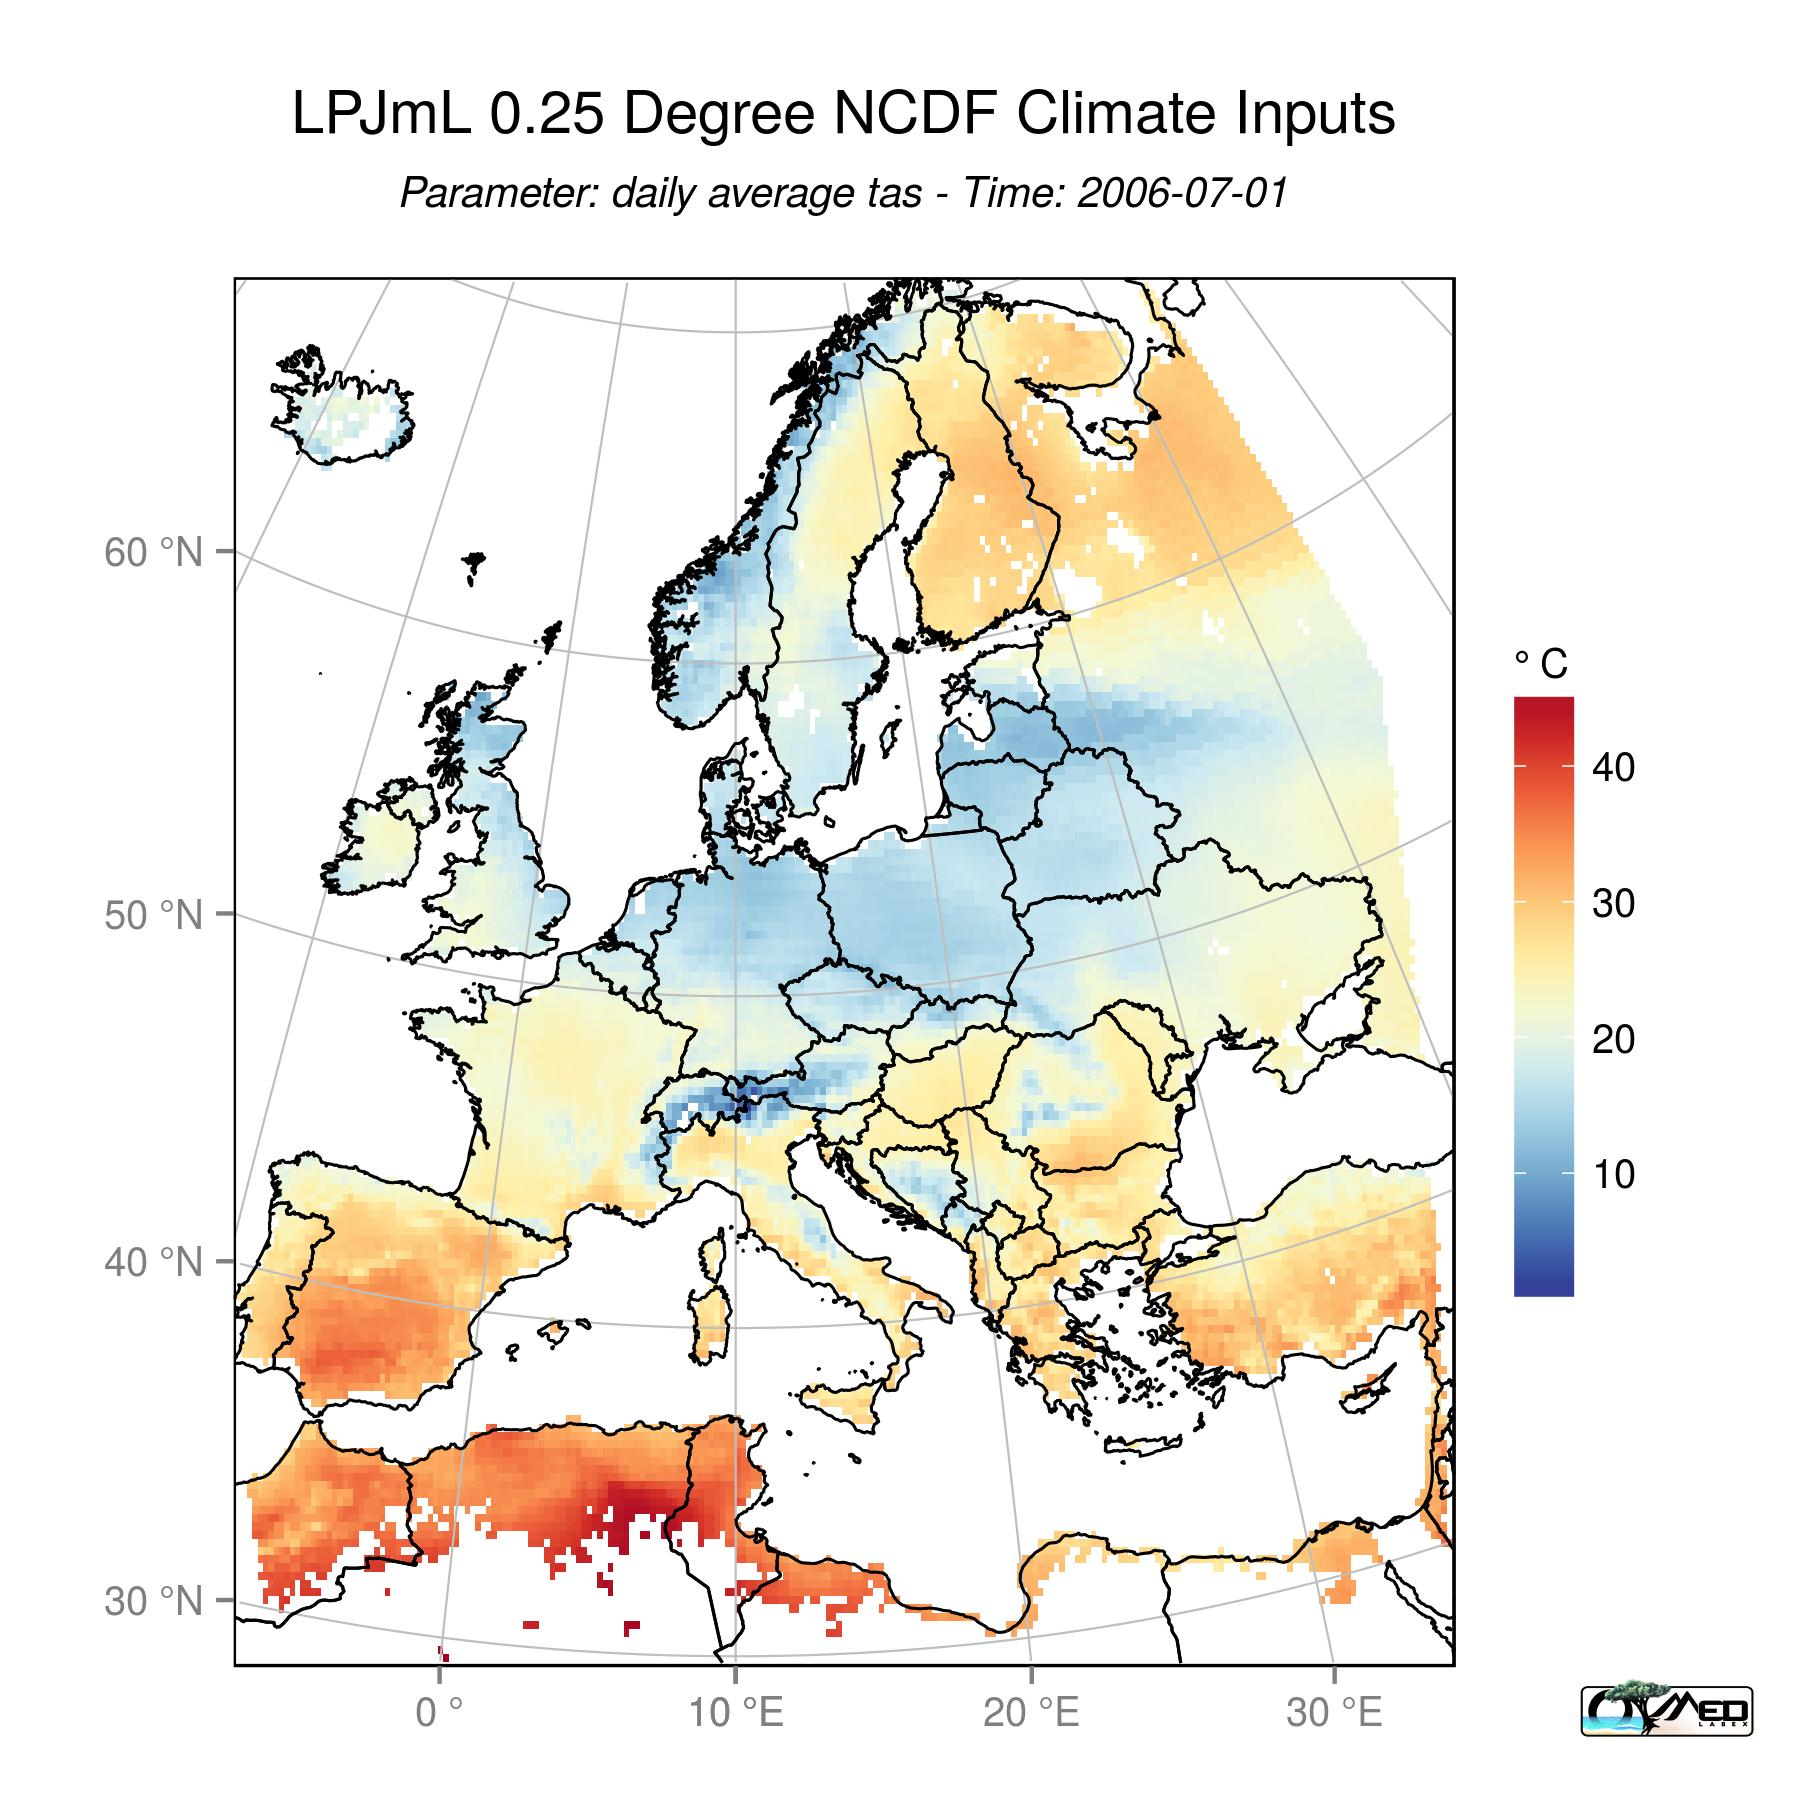
\includegraphics[width=0.45\textwidth, height=0.45\textwidth]{col2}
%   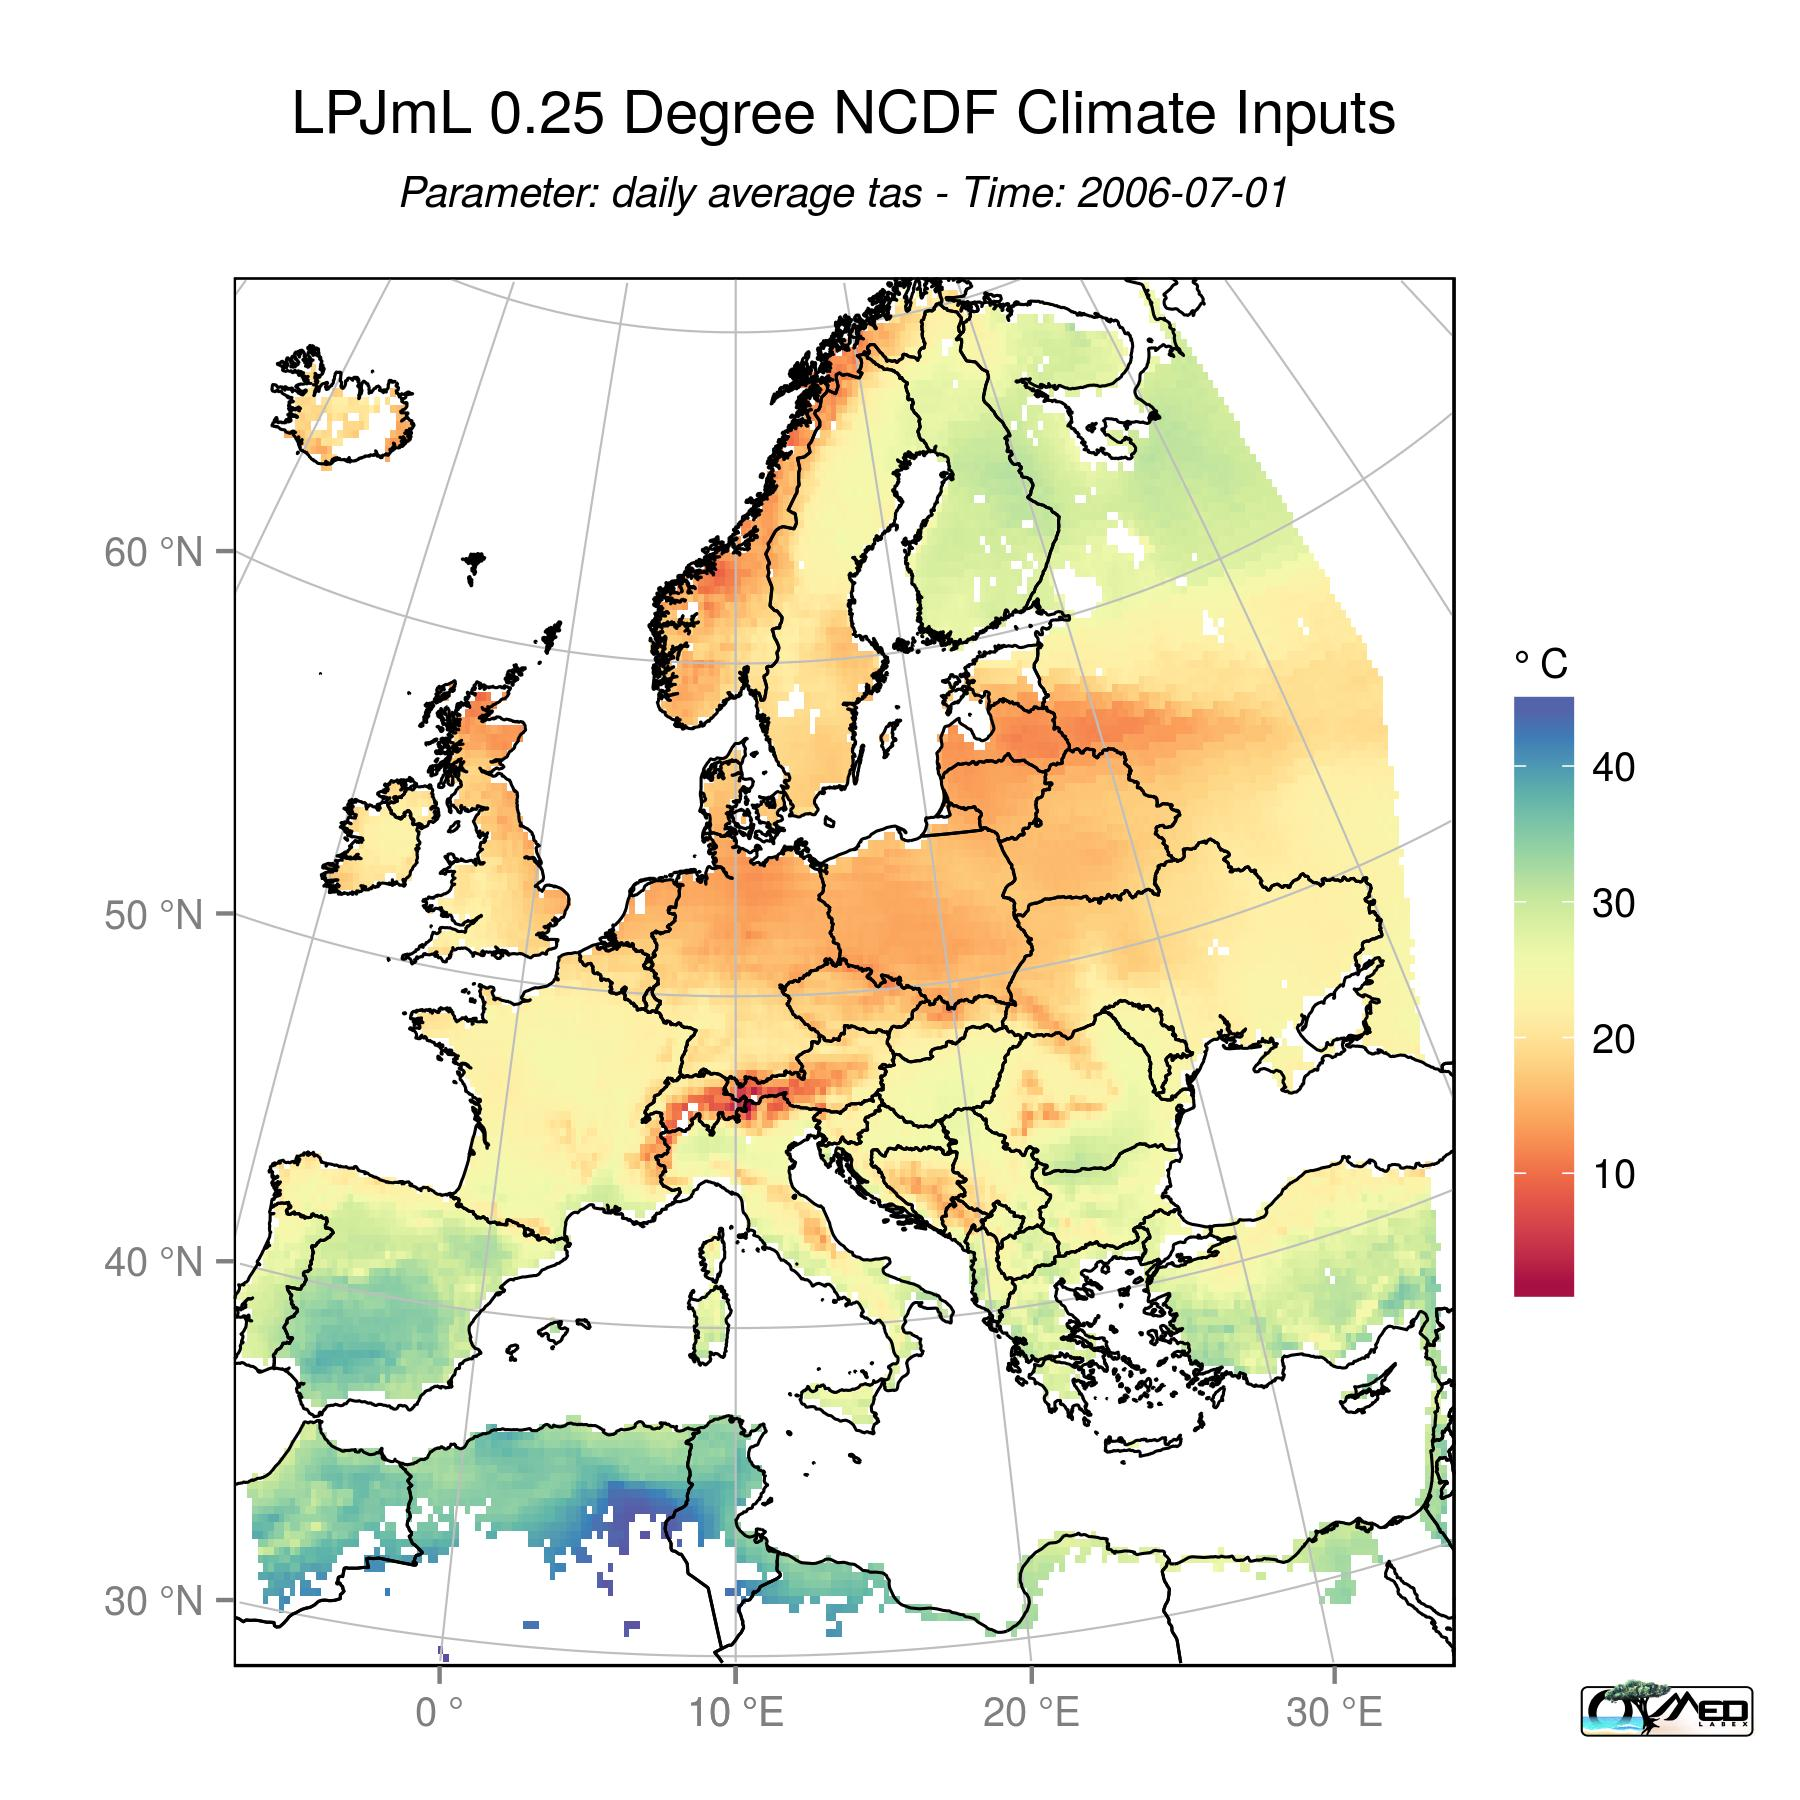
\includegraphics[width=0.45\textwidth, height=0.45\textwidth]{col4}
%   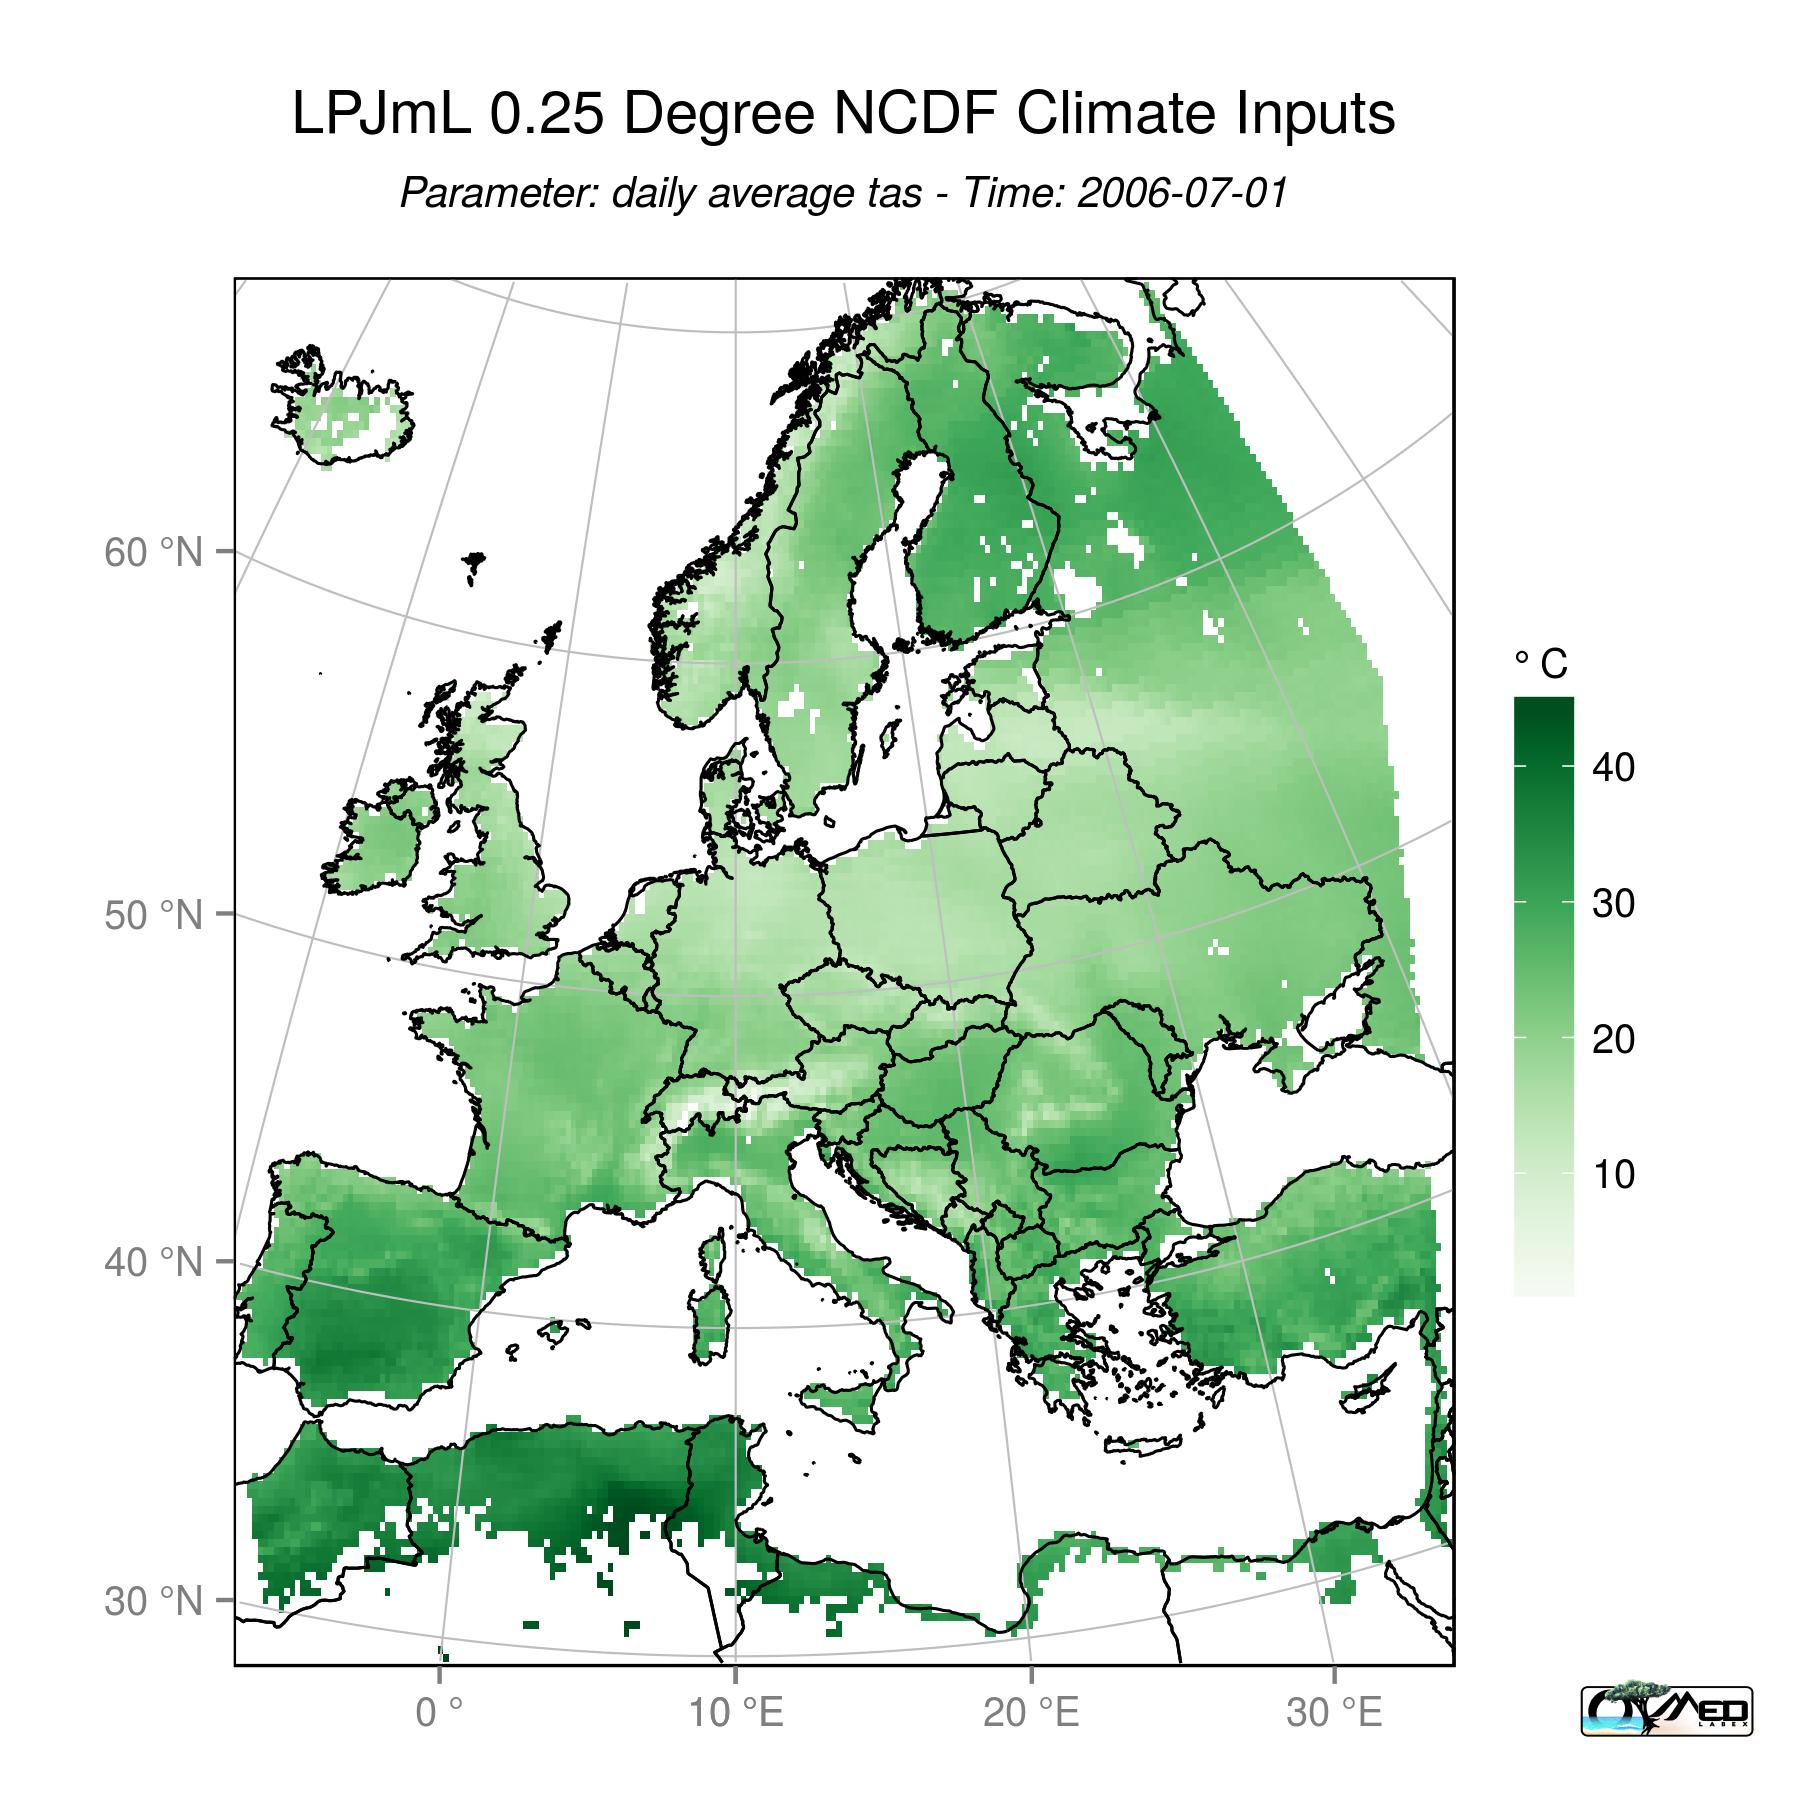
\includegraphics[width=0.45\textwidth, height=0.45\textwidth]{col_12}
%   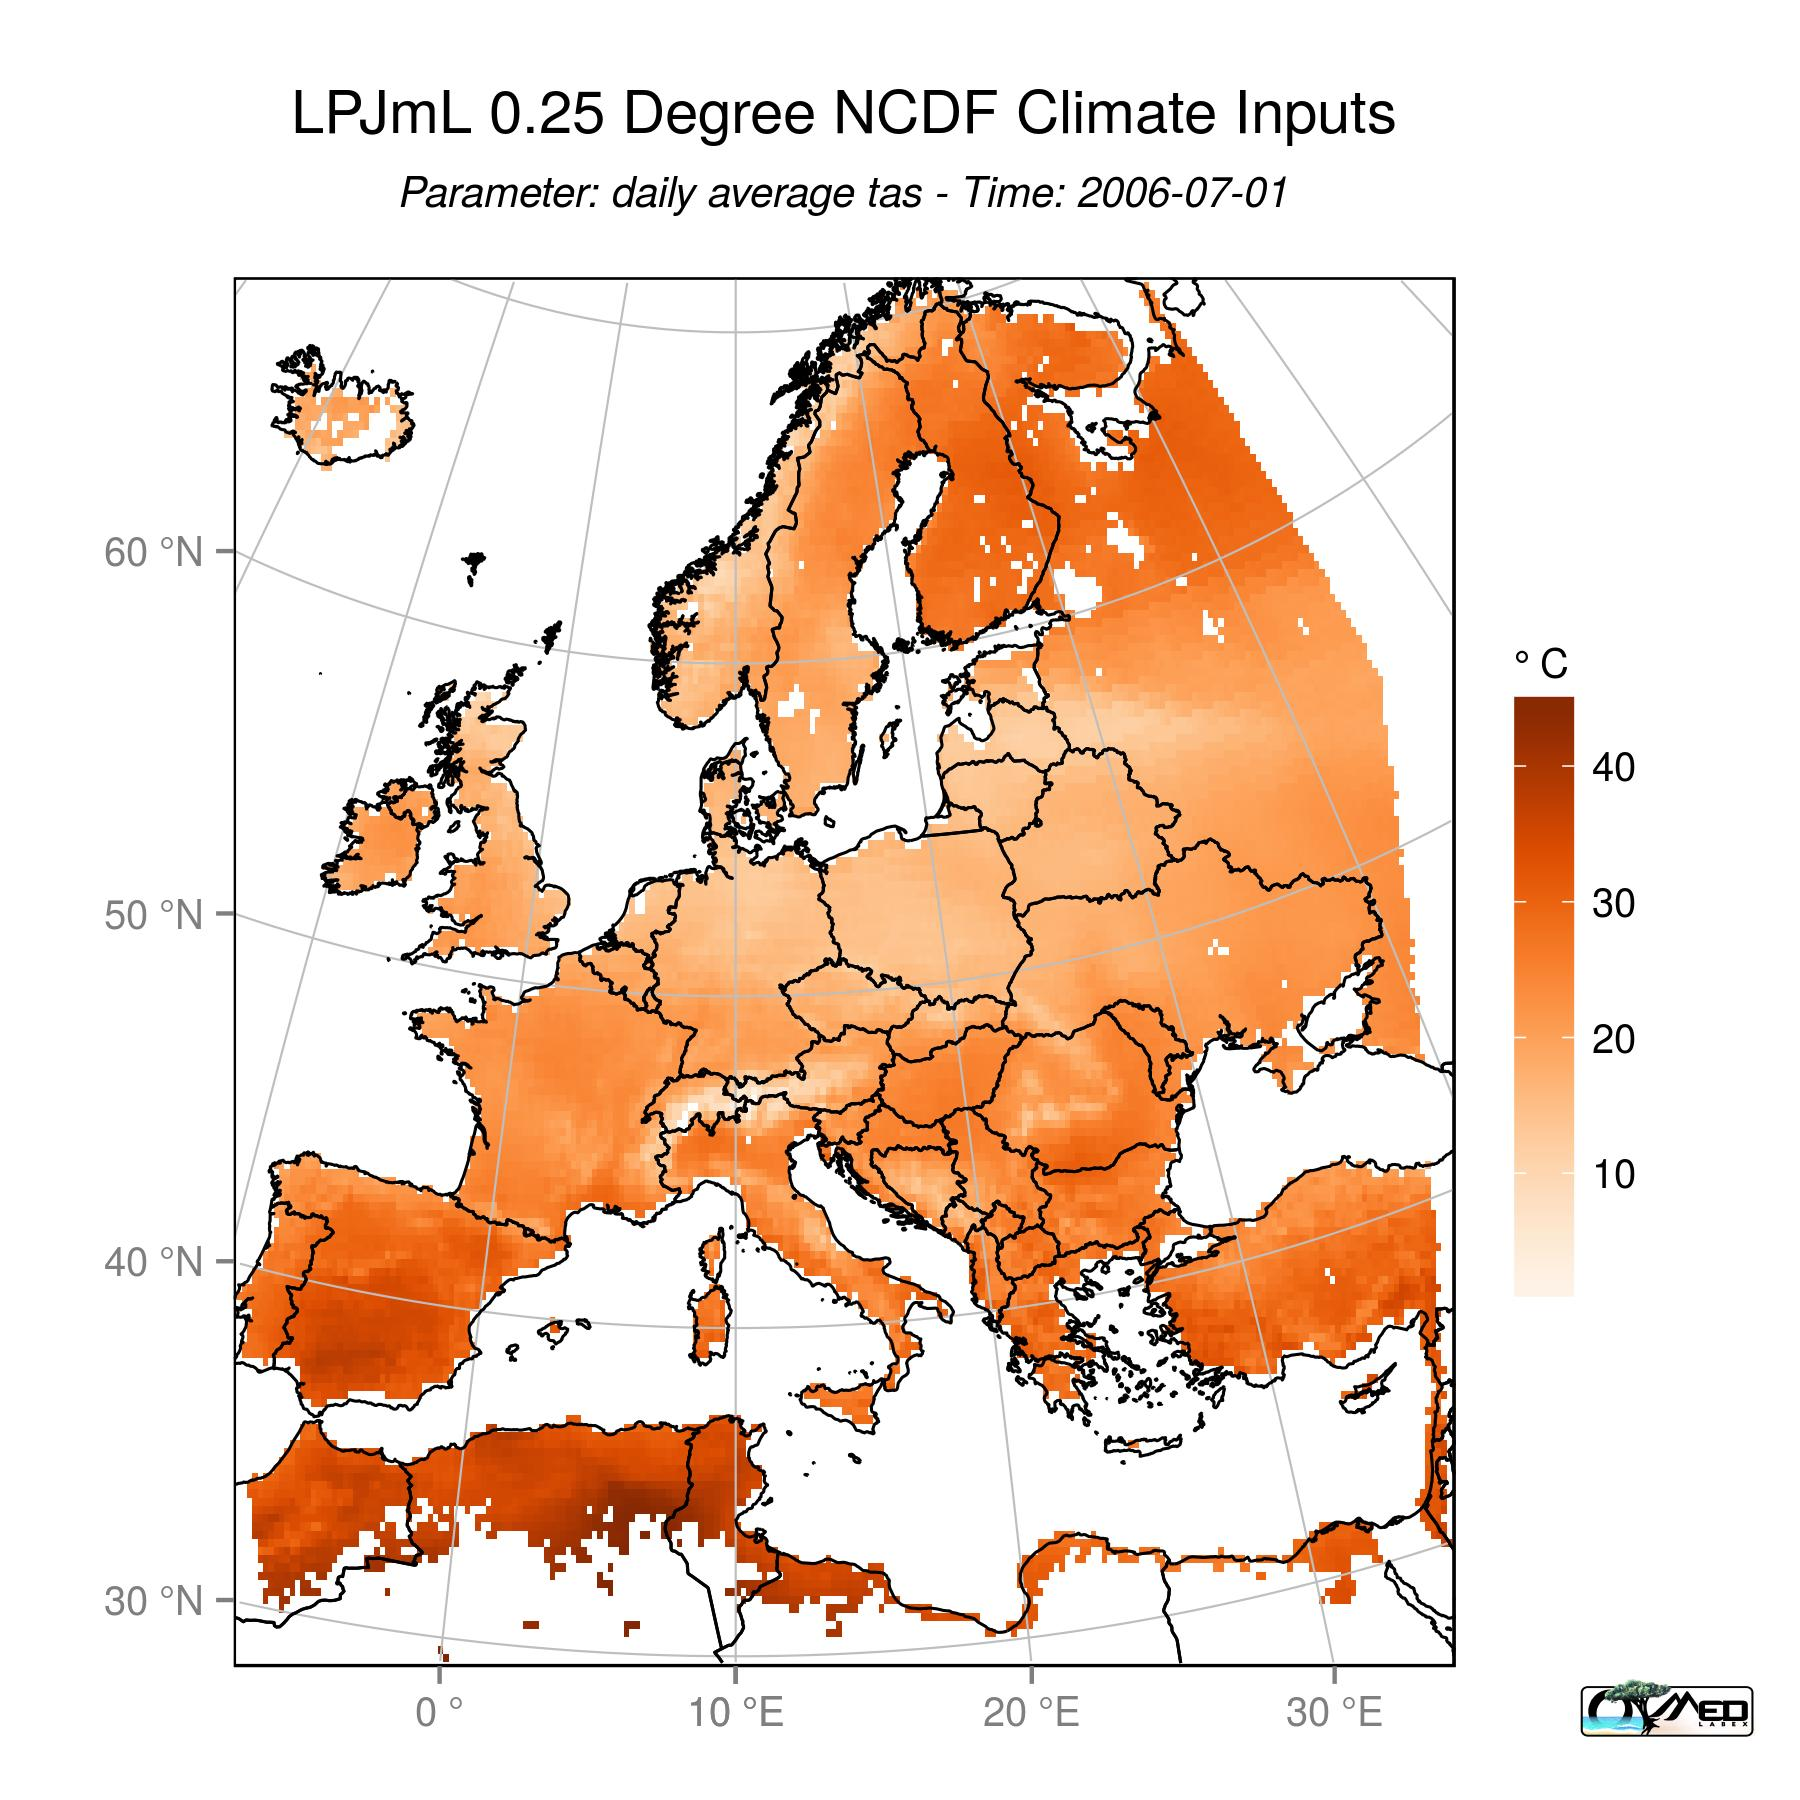
\includegraphics[width=0.45\textwidth, height=0.45\textwidth]{col_13}
%   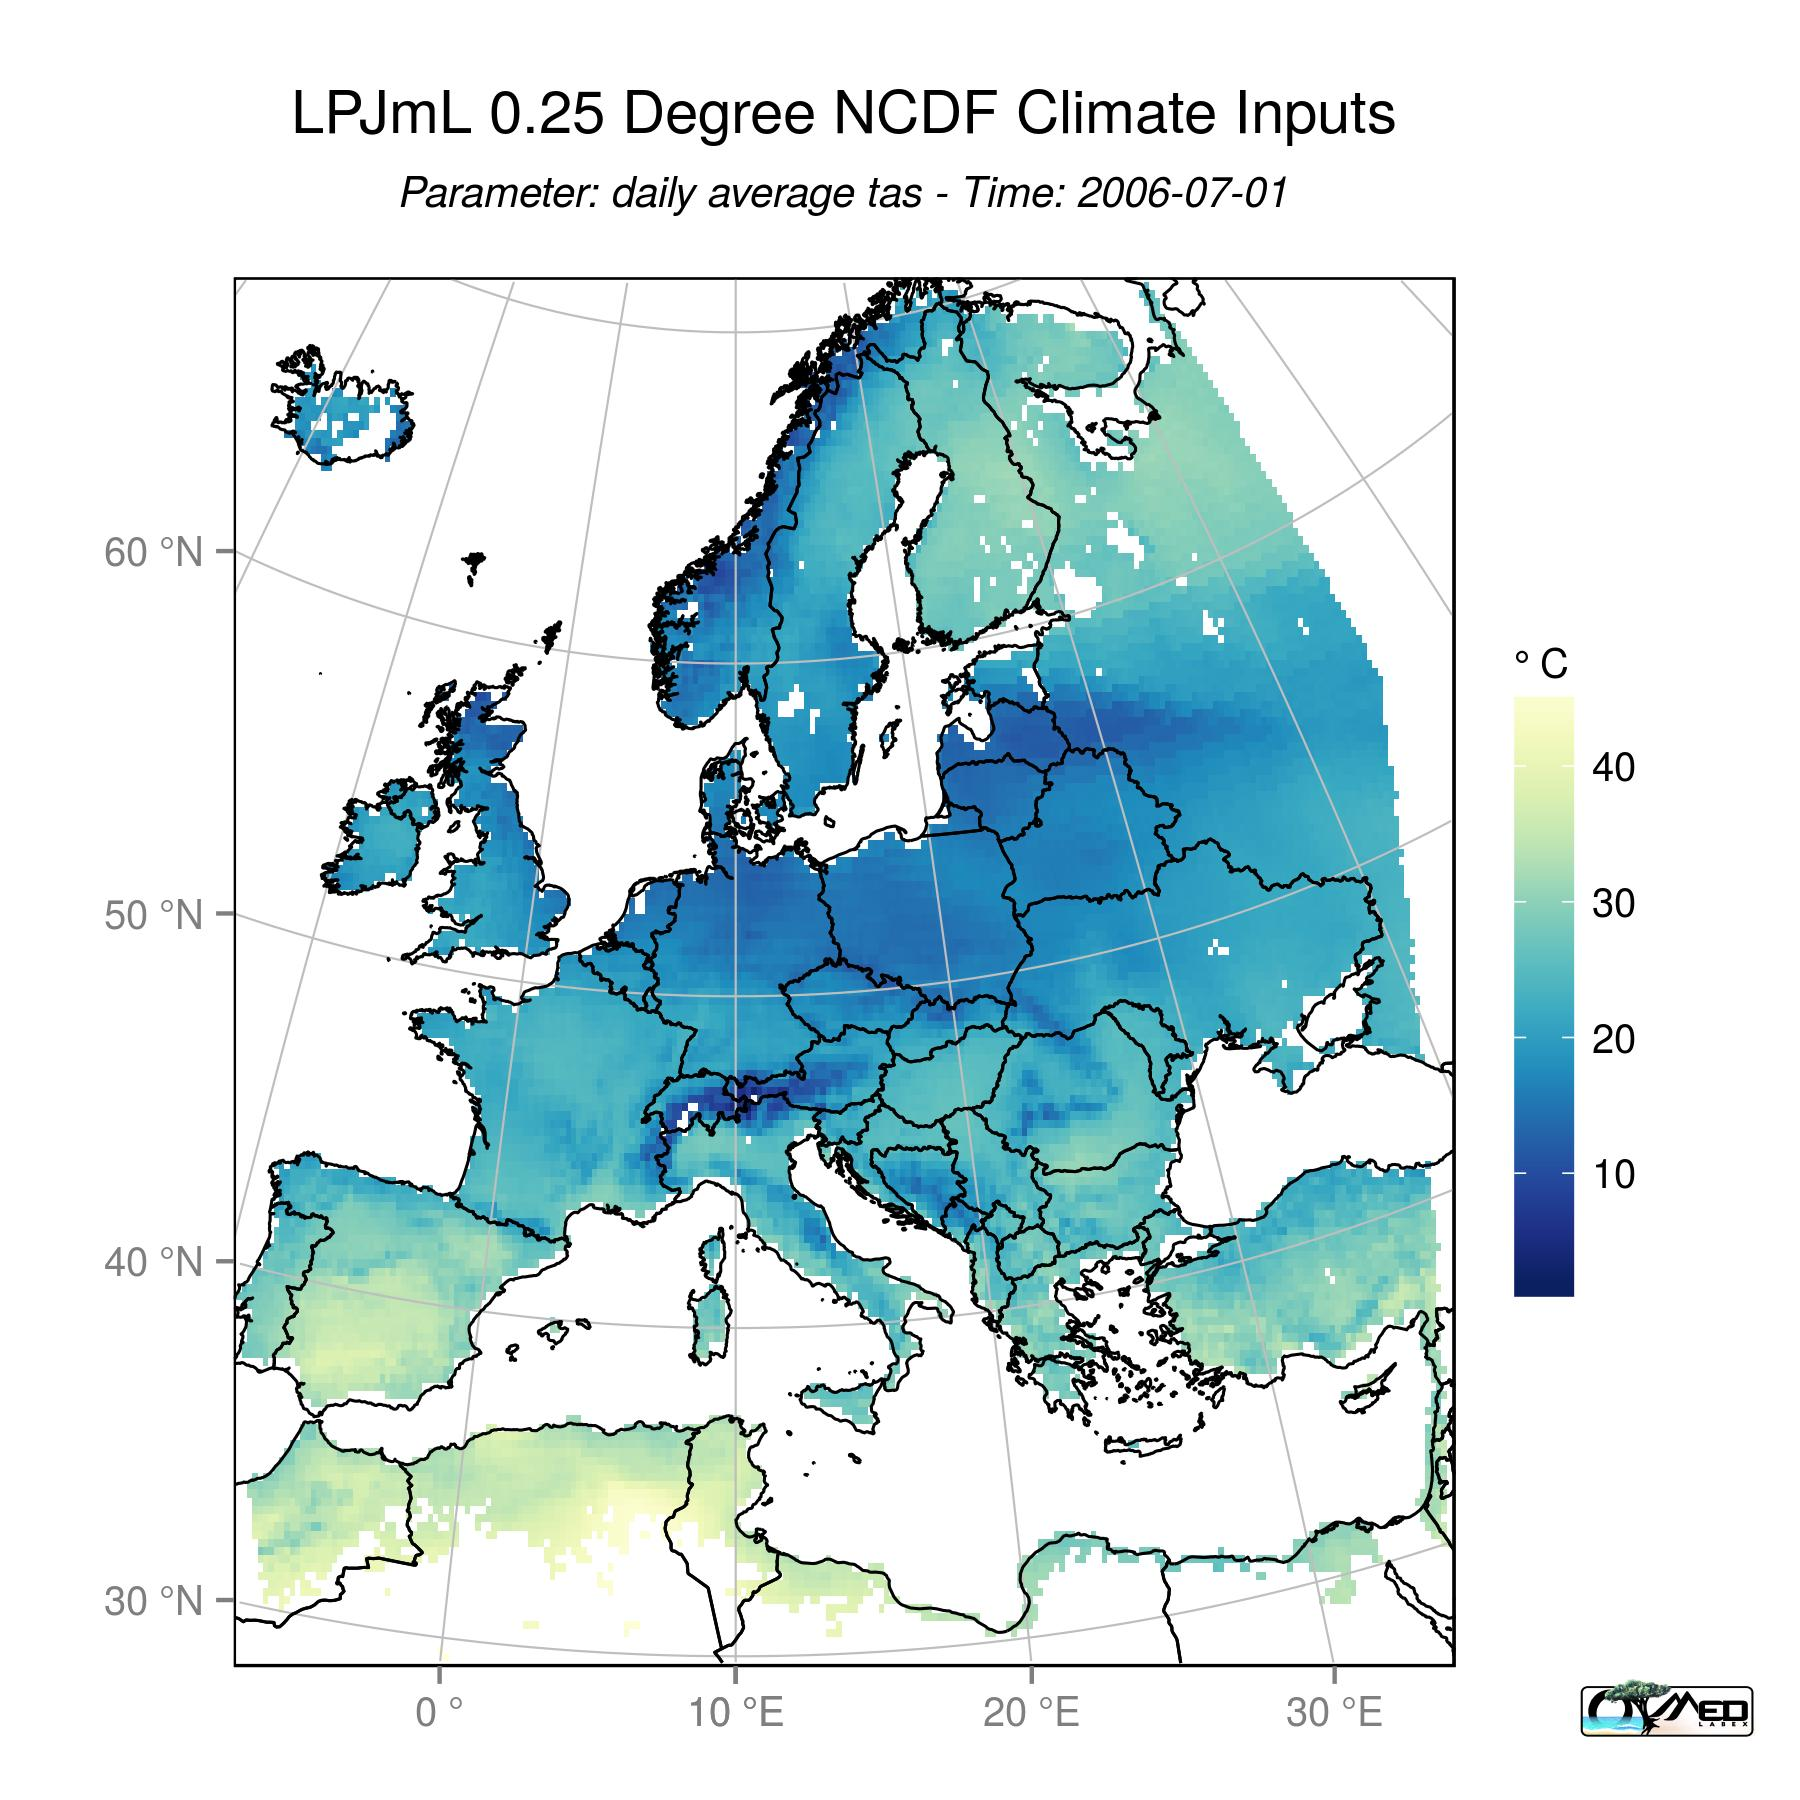
\includegraphics[width=0.45\textwidth, height=0.45\textwidth]{col_15}
%     \caption{Maps applied in different colour scales}
%   \label{fig:change color}
% \end{figure}
% 
% \subsection{Colour Bars Position}
% \subsection{Polygons Map}
% \section{Further Development}
% \subsection{Projection on irregular grids}
% 
% 
% 







\end{document}



